% Created by tikzDevice version 0.12 on 2019-05-09 12:20:37
% !TEX encoding = UTF-8 Unicode
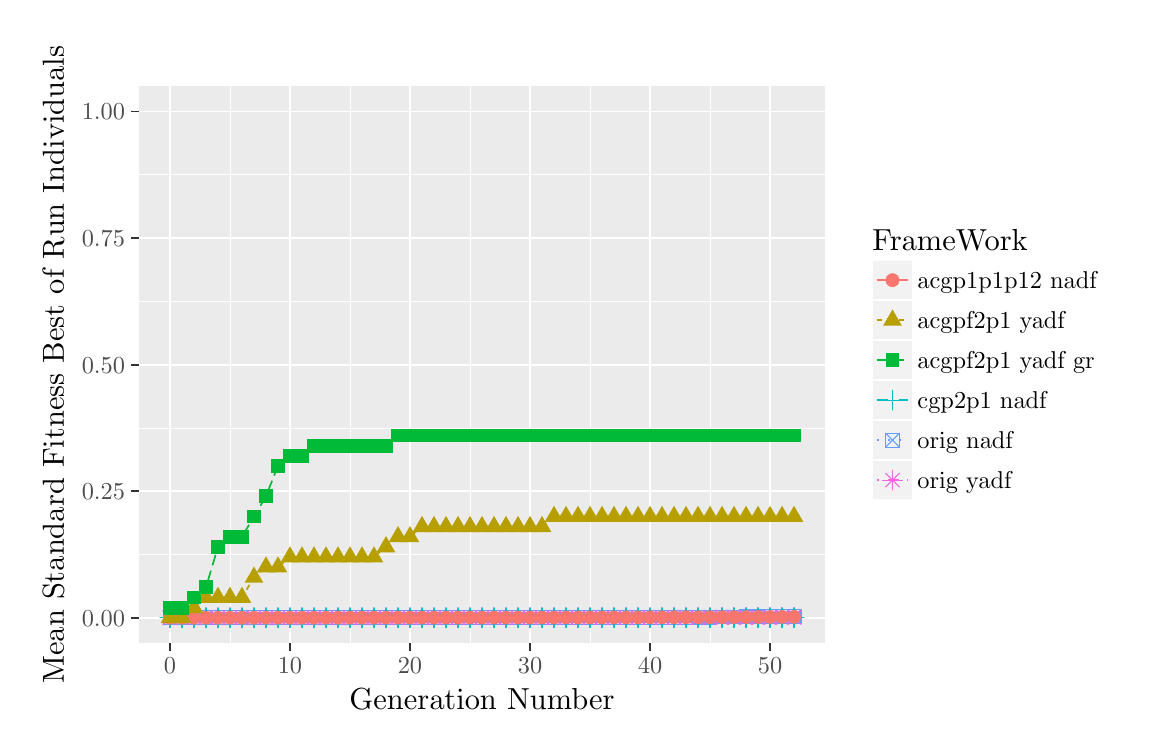
\begin{tikzpicture}[x=1pt,y=1pt]
\definecolor{fillColor}{RGB}{255,255,255}
\path[use as bounding box,fill=fillColor,fill opacity=0.00] (0,0) rectangle (397.48,252.94);
\begin{scope}
\path[clip] (  0.00,  0.00) rectangle (397.48,252.94);
\definecolor{drawColor}{RGB}{255,255,255}
\definecolor{fillColor}{RGB}{255,255,255}

\path[draw=drawColor,line width= 0.6pt,line join=round,line cap=round,fill=fillColor] (  0.00,  0.00) rectangle (397.48,252.95);
\end{scope}
\begin{scope}
\path[clip] ( 40.14, 30.56) rectangle (288.20,231.75);
\definecolor{fillColor}{gray}{0.92}

\path[fill=fillColor] ( 40.14, 30.56) rectangle (288.20,231.75);
\definecolor{drawColor}{RGB}{255,255,255}

\path[draw=drawColor,line width= 0.3pt,line join=round] ( 40.14, 62.57) --
	(288.20, 62.57);

\path[draw=drawColor,line width= 0.3pt,line join=round] ( 40.14,108.29) --
	(288.20,108.29);

\path[draw=drawColor,line width= 0.3pt,line join=round] ( 40.14,154.02) --
	(288.20,154.02);

\path[draw=drawColor,line width= 0.3pt,line join=round] ( 40.14,199.75) --
	(288.20,199.75);

\path[draw=drawColor,line width= 0.3pt,line join=round] ( 73.10, 30.56) --
	( 73.10,231.75);

\path[draw=drawColor,line width= 0.3pt,line join=round] (116.47, 30.56) --
	(116.47,231.75);

\path[draw=drawColor,line width= 0.3pt,line join=round] (159.83, 30.56) --
	(159.83,231.75);

\path[draw=drawColor,line width= 0.3pt,line join=round] (203.20, 30.56) --
	(203.20,231.75);

\path[draw=drawColor,line width= 0.3pt,line join=round] (246.57, 30.56) --
	(246.57,231.75);

\path[draw=drawColor,line width= 0.6pt,line join=round] ( 40.14, 39.70) --
	(288.20, 39.70);

\path[draw=drawColor,line width= 0.6pt,line join=round] ( 40.14, 85.43) --
	(288.20, 85.43);

\path[draw=drawColor,line width= 0.6pt,line join=round] ( 40.14,131.16) --
	(288.20,131.16);

\path[draw=drawColor,line width= 0.6pt,line join=round] ( 40.14,176.88) --
	(288.20,176.88);

\path[draw=drawColor,line width= 0.6pt,line join=round] ( 40.14,222.61) --
	(288.20,222.61);

\path[draw=drawColor,line width= 0.6pt,line join=round] ( 51.41, 30.56) --
	( 51.41,231.75);

\path[draw=drawColor,line width= 0.6pt,line join=round] ( 94.78, 30.56) --
	( 94.78,231.75);

\path[draw=drawColor,line width= 0.6pt,line join=round] (138.15, 30.56) --
	(138.15,231.75);

\path[draw=drawColor,line width= 0.6pt,line join=round] (181.52, 30.56) --
	(181.52,231.75);

\path[draw=drawColor,line width= 0.6pt,line join=round] (224.88, 30.56) --
	(224.88,231.75);

\path[draw=drawColor,line width= 0.6pt,line join=round] (268.25, 30.56) --
	(268.25,231.75);
\definecolor{drawColor}{RGB}{248,118,109}

\path[draw=drawColor,line width= 0.6pt,line join=round] ( 51.41, 39.71) --
	( 55.75, 39.71) --
	( 60.09, 39.71) --
	( 64.42, 39.71) --
	( 68.76, 39.71) --
	( 73.10, 39.71) --
	( 77.43, 39.71) --
	( 81.77, 39.71) --
	( 86.11, 39.72) --
	( 90.44, 39.72) --
	( 94.78, 39.72) --
	( 99.12, 39.72) --
	(103.45, 39.72) --
	(107.79, 39.72) --
	(112.13, 39.73) --
	(116.47, 39.73) --
	(120.80, 39.73) --
	(125.14, 39.73) --
	(129.48, 39.74) --
	(133.81, 39.74) --
	(138.15, 39.74) --
	(142.49, 39.74) --
	(146.82, 39.75) --
	(151.16, 39.75) --
	(155.50, 39.75) --
	(159.83, 39.76) --
	(164.17, 39.76) --
	(168.51, 39.77) --
	(172.84, 39.77) --
	(177.18, 39.77) --
	(181.52, 39.78) --
	(185.85, 39.78) --
	(190.19, 39.79) --
	(194.53, 39.80) --
	(198.86, 39.81) --
	(203.20, 39.82) --
	(207.54, 39.82) --
	(211.87, 39.83) --
	(216.21, 39.84) --
	(220.55, 39.85) --
	(224.88, 39.86) --
	(229.22, 39.87) --
	(233.56, 39.88) --
	(237.89, 39.89) --
	(242.23, 39.90) --
	(246.57, 39.92) --
	(250.90, 39.93) --
	(255.24, 39.94) --
	(259.58, 39.96) --
	(263.91, 39.98) --
	(268.25, 40.00) --
	(272.59, 40.02) --
	(276.92, 40.04);
\definecolor{drawColor}{RGB}{183,159,0}

\path[draw=drawColor,line width= 0.6pt,dash pattern=on 2pt off 2pt ,line join=round] ( 51.41, 39.71) --
	( 55.75, 39.71) --
	( 60.09, 43.37) --
	( 64.42, 47.03) --
	( 68.76, 47.03) --
	( 73.10, 47.03) --
	( 77.43, 47.03) --
	( 81.77, 54.35) --
	( 86.11, 58.01) --
	( 90.44, 58.01) --
	( 94.78, 61.67) --
	( 99.12, 61.67) --
	(103.45, 61.67) --
	(107.79, 61.67) --
	(112.13, 61.67) --
	(116.47, 61.67) --
	(120.80, 61.67) --
	(125.14, 61.67) --
	(129.48, 65.32) --
	(133.81, 68.98) --
	(138.15, 68.98) --
	(142.49, 72.64) --
	(146.82, 72.64) --
	(151.16, 72.64) --
	(155.50, 72.64) --
	(159.83, 72.64) --
	(164.17, 72.64) --
	(168.51, 72.64) --
	(172.84, 72.64) --
	(177.18, 72.64) --
	(181.52, 72.64) --
	(185.85, 72.64) --
	(190.19, 76.30) --
	(194.53, 76.30) --
	(198.86, 76.30) --
	(203.20, 76.30) --
	(207.54, 76.30) --
	(211.87, 76.30) --
	(216.21, 76.30) --
	(220.55, 76.30) --
	(224.88, 76.30) --
	(229.22, 76.30) --
	(233.56, 76.30) --
	(237.89, 76.30) --
	(242.23, 76.30) --
	(246.57, 76.30) --
	(250.90, 76.30) --
	(255.24, 76.30) --
	(259.58, 76.30) --
	(263.91, 76.30) --
	(268.25, 76.30) --
	(272.59, 76.30) --
	(276.92, 76.30);
\definecolor{drawColor}{RGB}{0,186,56}

\path[draw=drawColor,line width= 0.6pt,dash pattern=on 4pt off 2pt ,line join=round] ( 51.41, 43.37) --
	( 55.75, 43.37) --
	( 60.09, 47.03) --
	( 64.42, 50.69) --
	( 68.76, 65.32) --
	( 73.10, 68.98) --
	( 77.43, 68.98) --
	( 81.77, 76.30) --
	( 86.11, 83.61) --
	( 90.44, 94.59) --
	( 94.78, 98.24) --
	( 99.12, 98.24) --
	(103.45,101.90) --
	(107.79,101.90) --
	(112.13,101.90) --
	(116.47,101.90) --
	(120.80,101.90) --
	(125.14,101.90) --
	(129.48,101.90) --
	(133.81,105.56) --
	(138.15,105.56) --
	(142.49,105.56) --
	(146.82,105.56) --
	(151.16,105.56) --
	(155.50,105.56) --
	(159.83,105.56) --
	(164.17,105.56) --
	(168.51,105.56) --
	(172.84,105.56) --
	(177.18,105.56) --
	(181.52,105.56) --
	(185.85,105.56) --
	(190.19,105.56) --
	(194.53,105.56) --
	(198.86,105.56) --
	(203.20,105.56) --
	(207.54,105.56) --
	(211.87,105.56) --
	(216.21,105.56) --
	(220.55,105.56) --
	(224.88,105.56) --
	(229.22,105.56) --
	(233.56,105.56) --
	(237.89,105.56) --
	(242.23,105.56) --
	(246.57,105.56) --
	(250.90,105.56) --
	(255.24,105.56) --
	(259.58,105.56) --
	(263.91,105.56) --
	(268.25,105.56) --
	(272.59,105.56) --
	(276.92,105.56);
\definecolor{drawColor}{RGB}{0,191,196}

\path[draw=drawColor,line width= 0.6pt,dash pattern=on 4pt off 4pt ,line join=round] ( 51.41, 39.70) --
	( 55.75, 39.70) --
	( 60.09, 39.70) --
	( 64.42, 39.70) --
	( 68.76, 39.70) --
	( 73.10, 39.70) --
	( 77.43, 39.70) --
	( 81.77, 39.70) --
	( 86.11, 39.70) --
	( 90.44, 39.70) --
	( 94.78, 39.70) --
	( 99.12, 39.70) --
	(103.45, 39.70) --
	(107.79, 39.70) --
	(112.13, 39.70) --
	(116.47, 39.70) --
	(120.80, 39.70) --
	(125.14, 39.70) --
	(129.48, 39.70) --
	(133.81, 39.70) --
	(138.15, 39.70) --
	(142.49, 39.70) --
	(146.82, 39.70) --
	(151.16, 39.70) --
	(155.50, 39.70) --
	(159.83, 39.70) --
	(164.17, 39.70) --
	(168.51, 39.70) --
	(172.84, 39.70) --
	(177.18, 39.70) --
	(181.52, 39.70) --
	(185.85, 39.70) --
	(190.19, 39.70) --
	(194.53, 39.70) --
	(198.86, 39.70) --
	(203.20, 39.70) --
	(207.54, 39.70) --
	(211.87, 39.70) --
	(216.21, 39.70) --
	(220.55, 39.70) --
	(224.88, 39.70) --
	(229.22, 39.70) --
	(233.56, 39.70) --
	(237.89, 39.70) --
	(242.23, 39.70) --
	(246.57, 39.70) --
	(250.90, 39.70) --
	(255.24, 39.70) --
	(259.58, 39.70) --
	(263.91, 39.70) --
	(268.25, 39.70) --
	(272.59, 39.70) --
	(276.92, 39.70);
\definecolor{drawColor}{RGB}{97,156,255}

\path[draw=drawColor,line width= 0.6pt,dash pattern=on 1pt off 3pt ,line join=round] ( 51.41, 39.71) --
	( 55.75, 39.71) --
	( 60.09, 39.71) --
	( 64.42, 39.71) --
	( 68.76, 39.71) --
	( 73.10, 39.71) --
	( 77.43, 39.71) --
	( 81.77, 39.72) --
	( 86.11, 39.72) --
	( 90.44, 39.72) --
	( 94.78, 39.72) --
	( 99.12, 39.72) --
	(103.45, 39.73) --
	(107.79, 39.73) --
	(112.13, 39.73) --
	(116.47, 39.73) --
	(120.80, 39.73) --
	(125.14, 39.74) --
	(129.48, 39.74) --
	(133.81, 39.74) --
	(138.15, 39.75) --
	(142.49, 39.75) --
	(146.82, 39.75) --
	(151.16, 39.76) --
	(155.50, 39.76) --
	(159.83, 39.77) --
	(164.17, 39.77) --
	(168.51, 39.78) --
	(172.84, 39.78) --
	(177.18, 39.79) --
	(181.52, 39.79) --
	(185.85, 39.80) --
	(190.19, 39.81) --
	(194.53, 39.82) --
	(198.86, 39.83) --
	(203.20, 39.84) --
	(207.54, 39.85) --
	(211.87, 39.86) --
	(216.21, 39.87) --
	(220.55, 39.88) --
	(224.88, 39.89) --
	(229.22, 39.90) --
	(233.56, 39.92) --
	(237.89, 39.93) --
	(242.23, 39.95) --
	(246.57, 39.96) --
	(250.90, 39.98) --
	(255.24, 39.99) --
	(259.58, 40.01) --
	(263.91, 40.03) --
	(268.25, 40.05) --
	(272.59, 40.08) --
	(276.92, 40.10);
\definecolor{drawColor}{RGB}{245,100,227}

\path[draw=drawColor,line width= 0.6pt,dash pattern=on 1pt off 3pt on 4pt off 3pt ,line join=round] ( 51.41, 39.71) --
	( 55.75, 39.71) --
	( 60.09, 39.71) --
	( 64.42, 39.71) --
	( 68.76, 39.71) --
	( 73.10, 39.71) --
	( 77.43, 39.71) --
	( 81.77, 39.71) --
	( 86.11, 39.71) --
	( 90.44, 39.71) --
	( 94.78, 39.72) --
	( 99.12, 39.72) --
	(103.45, 39.72) --
	(107.79, 39.72) --
	(112.13, 39.72) --
	(116.47, 39.72) --
	(120.80, 39.72) --
	(125.14, 39.72) --
	(129.48, 39.72) --
	(133.81, 39.73) --
	(138.15, 39.73) --
	(142.49, 39.73) --
	(146.82, 39.73) --
	(151.16, 39.73) --
	(155.50, 39.73) --
	(159.83, 39.73) --
	(164.17, 39.74) --
	(168.51, 39.74) --
	(172.84, 39.74) --
	(177.18, 39.74) --
	(181.52, 39.74) --
	(185.85, 39.75) --
	(190.19, 39.75) --
	(194.53, 39.75) --
	(198.86, 39.75) --
	(203.20, 39.75) --
	(207.54, 39.76) --
	(211.87, 39.76) --
	(216.21, 39.76) --
	(220.55, 39.76) --
	(224.88, 39.77) --
	(229.22, 39.77) --
	(233.56, 39.77) --
	(237.89, 39.78) --
	(242.23, 39.78) --
	(246.57, 39.79) --
	(250.90, 39.79) --
	(255.24, 39.80) --
	(259.58, 39.80) --
	(263.91, 39.80) --
	(268.25, 39.81) --
	(272.59, 39.81) --
	(276.92, 39.82);
\definecolor{drawColor}{RGB}{97,156,255}

\path[draw=drawColor,line width= 0.4pt,line join=round,line cap=round] ( 48.92, 37.21) rectangle ( 53.91, 42.20);

\path[draw=drawColor,line width= 0.4pt,line join=round,line cap=round] ( 48.92, 37.21) -- ( 53.91, 42.20);

\path[draw=drawColor,line width= 0.4pt,line join=round,line cap=round] ( 48.92, 42.20) -- ( 53.91, 37.21);

\path[draw=drawColor,line width= 0.4pt,line join=round,line cap=round] ( 53.25, 37.21) rectangle ( 58.25, 42.20);

\path[draw=drawColor,line width= 0.4pt,line join=round,line cap=round] ( 53.25, 37.21) -- ( 58.25, 42.20);

\path[draw=drawColor,line width= 0.4pt,line join=round,line cap=round] ( 53.25, 42.20) -- ( 58.25, 37.21);

\path[draw=drawColor,line width= 0.4pt,line join=round,line cap=round] ( 57.59, 37.21) rectangle ( 62.59, 42.21);

\path[draw=drawColor,line width= 0.4pt,line join=round,line cap=round] ( 57.59, 37.21) -- ( 62.59, 42.21);

\path[draw=drawColor,line width= 0.4pt,line join=round,line cap=round] ( 57.59, 42.21) -- ( 62.59, 37.21);

\path[draw=drawColor,line width= 0.4pt,line join=round,line cap=round] ( 61.93, 37.21) rectangle ( 66.92, 42.21);

\path[draw=drawColor,line width= 0.4pt,line join=round,line cap=round] ( 61.93, 37.21) -- ( 66.92, 42.21);

\path[draw=drawColor,line width= 0.4pt,line join=round,line cap=round] ( 61.93, 42.21) -- ( 66.92, 37.21);

\path[draw=drawColor,line width= 0.4pt,line join=round,line cap=round] ( 66.26, 37.21) rectangle ( 71.26, 42.21);

\path[draw=drawColor,line width= 0.4pt,line join=round,line cap=round] ( 66.26, 37.21) -- ( 71.26, 42.21);

\path[draw=drawColor,line width= 0.4pt,line join=round,line cap=round] ( 66.26, 42.21) -- ( 71.26, 37.21);

\path[draw=drawColor,line width= 0.4pt,line join=round,line cap=round] ( 70.60, 37.22) rectangle ( 75.60, 42.21);

\path[draw=drawColor,line width= 0.4pt,line join=round,line cap=round] ( 70.60, 37.22) -- ( 75.60, 42.21);

\path[draw=drawColor,line width= 0.4pt,line join=round,line cap=round] ( 70.60, 42.21) -- ( 75.60, 37.22);

\path[draw=drawColor,line width= 0.4pt,line join=round,line cap=round] ( 74.94, 37.22) rectangle ( 79.93, 42.21);

\path[draw=drawColor,line width= 0.4pt,line join=round,line cap=round] ( 74.94, 37.22) -- ( 79.93, 42.21);

\path[draw=drawColor,line width= 0.4pt,line join=round,line cap=round] ( 74.94, 42.21) -- ( 79.93, 37.22);

\path[draw=drawColor,line width= 0.4pt,line join=round,line cap=round] ( 79.27, 37.22) rectangle ( 84.27, 42.21);

\path[draw=drawColor,line width= 0.4pt,line join=round,line cap=round] ( 79.27, 37.22) -- ( 84.27, 42.21);

\path[draw=drawColor,line width= 0.4pt,line join=round,line cap=round] ( 79.27, 42.21) -- ( 84.27, 37.22);

\path[draw=drawColor,line width= 0.4pt,line join=round,line cap=round] ( 83.61, 37.22) rectangle ( 88.61, 42.22);

\path[draw=drawColor,line width= 0.4pt,line join=round,line cap=round] ( 83.61, 37.22) -- ( 88.61, 42.22);

\path[draw=drawColor,line width= 0.4pt,line join=round,line cap=round] ( 83.61, 42.22) -- ( 88.61, 37.22);

\path[draw=drawColor,line width= 0.4pt,line join=round,line cap=round] ( 87.95, 37.22) rectangle ( 92.94, 42.22);

\path[draw=drawColor,line width= 0.4pt,line join=round,line cap=round] ( 87.95, 37.22) -- ( 92.94, 42.22);

\path[draw=drawColor,line width= 0.4pt,line join=round,line cap=round] ( 87.95, 42.22) -- ( 92.94, 37.22);

\path[draw=drawColor,line width= 0.4pt,line join=round,line cap=round] ( 92.28, 37.22) rectangle ( 97.28, 42.22);

\path[draw=drawColor,line width= 0.4pt,line join=round,line cap=round] ( 92.28, 37.22) -- ( 97.28, 42.22);

\path[draw=drawColor,line width= 0.4pt,line join=round,line cap=round] ( 92.28, 42.22) -- ( 97.28, 37.22);

\path[draw=drawColor,line width= 0.4pt,line join=round,line cap=round] ( 96.62, 37.23) rectangle (101.62, 42.22);

\path[draw=drawColor,line width= 0.4pt,line join=round,line cap=round] ( 96.62, 37.23) -- (101.62, 42.22);

\path[draw=drawColor,line width= 0.4pt,line join=round,line cap=round] ( 96.62, 42.22) -- (101.62, 37.23);

\path[draw=drawColor,line width= 0.4pt,line join=round,line cap=round] (100.96, 37.23) rectangle (105.95, 42.22);

\path[draw=drawColor,line width= 0.4pt,line join=round,line cap=round] (100.96, 37.23) -- (105.95, 42.22);

\path[draw=drawColor,line width= 0.4pt,line join=round,line cap=round] (100.96, 42.22) -- (105.95, 37.23);

\path[draw=drawColor,line width= 0.4pt,line join=round,line cap=round] (105.29, 37.23) rectangle (110.29, 42.23);

\path[draw=drawColor,line width= 0.4pt,line join=round,line cap=round] (105.29, 37.23) -- (110.29, 42.23);

\path[draw=drawColor,line width= 0.4pt,line join=round,line cap=round] (105.29, 42.23) -- (110.29, 37.23);

\path[draw=drawColor,line width= 0.4pt,line join=round,line cap=round] (109.63, 37.23) rectangle (114.63, 42.23);

\path[draw=drawColor,line width= 0.4pt,line join=round,line cap=round] (109.63, 37.23) -- (114.63, 42.23);

\path[draw=drawColor,line width= 0.4pt,line join=round,line cap=round] (109.63, 42.23) -- (114.63, 37.23);

\path[draw=drawColor,line width= 0.4pt,line join=round,line cap=round] (113.97, 37.24) rectangle (118.96, 42.23);

\path[draw=drawColor,line width= 0.4pt,line join=round,line cap=round] (113.97, 37.24) -- (118.96, 42.23);

\path[draw=drawColor,line width= 0.4pt,line join=round,line cap=round] (113.97, 42.23) -- (118.96, 37.24);

\path[draw=drawColor,line width= 0.4pt,line join=round,line cap=round] (118.30, 37.24) rectangle (123.30, 42.23);

\path[draw=drawColor,line width= 0.4pt,line join=round,line cap=round] (118.30, 37.24) -- (123.30, 42.23);

\path[draw=drawColor,line width= 0.4pt,line join=round,line cap=round] (118.30, 42.23) -- (123.30, 37.24);

\path[draw=drawColor,line width= 0.4pt,line join=round,line cap=round] (122.64, 37.24) rectangle (127.64, 42.23);

\path[draw=drawColor,line width= 0.4pt,line join=round,line cap=round] (122.64, 37.24) -- (127.64, 42.23);

\path[draw=drawColor,line width= 0.4pt,line join=round,line cap=round] (122.64, 42.23) -- (127.64, 37.24);

\path[draw=drawColor,line width= 0.4pt,line join=round,line cap=round] (126.98, 37.24) rectangle (131.97, 42.24);

\path[draw=drawColor,line width= 0.4pt,line join=round,line cap=round] (126.98, 37.24) -- (131.97, 42.24);

\path[draw=drawColor,line width= 0.4pt,line join=round,line cap=round] (126.98, 42.24) -- (131.97, 37.24);

\path[draw=drawColor,line width= 0.4pt,line join=round,line cap=round] (131.31, 37.24) rectangle (136.31, 42.24);

\path[draw=drawColor,line width= 0.4pt,line join=round,line cap=round] (131.31, 37.24) -- (136.31, 42.24);

\path[draw=drawColor,line width= 0.4pt,line join=round,line cap=round] (131.31, 42.24) -- (136.31, 37.24);

\path[draw=drawColor,line width= 0.4pt,line join=round,line cap=round] (135.65, 37.25) rectangle (140.65, 42.24);

\path[draw=drawColor,line width= 0.4pt,line join=round,line cap=round] (135.65, 37.25) -- (140.65, 42.24);

\path[draw=drawColor,line width= 0.4pt,line join=round,line cap=round] (135.65, 42.24) -- (140.65, 37.25);

\path[draw=drawColor,line width= 0.4pt,line join=round,line cap=round] (139.99, 37.25) rectangle (144.98, 42.25);

\path[draw=drawColor,line width= 0.4pt,line join=round,line cap=round] (139.99, 37.25) -- (144.98, 42.25);

\path[draw=drawColor,line width= 0.4pt,line join=round,line cap=round] (139.99, 42.25) -- (144.98, 37.25);

\path[draw=drawColor,line width= 0.4pt,line join=round,line cap=round] (144.32, 37.26) rectangle (149.32, 42.25);

\path[draw=drawColor,line width= 0.4pt,line join=round,line cap=round] (144.32, 37.26) -- (149.32, 42.25);

\path[draw=drawColor,line width= 0.4pt,line join=round,line cap=round] (144.32, 42.25) -- (149.32, 37.26);

\path[draw=drawColor,line width= 0.4pt,line join=round,line cap=round] (148.66, 37.26) rectangle (153.66, 42.26);

\path[draw=drawColor,line width= 0.4pt,line join=round,line cap=round] (148.66, 37.26) -- (153.66, 42.26);

\path[draw=drawColor,line width= 0.4pt,line join=round,line cap=round] (148.66, 42.26) -- (153.66, 37.26);

\path[draw=drawColor,line width= 0.4pt,line join=round,line cap=round] (153.00, 37.26) rectangle (157.99, 42.26);

\path[draw=drawColor,line width= 0.4pt,line join=round,line cap=round] (153.00, 37.26) -- (157.99, 42.26);

\path[draw=drawColor,line width= 0.4pt,line join=round,line cap=round] (153.00, 42.26) -- (157.99, 37.26);

\path[draw=drawColor,line width= 0.4pt,line join=round,line cap=round] (157.33, 37.27) rectangle (162.33, 42.26);

\path[draw=drawColor,line width= 0.4pt,line join=round,line cap=round] (157.33, 37.27) -- (162.33, 42.26);

\path[draw=drawColor,line width= 0.4pt,line join=round,line cap=round] (157.33, 42.26) -- (162.33, 37.27);

\path[draw=drawColor,line width= 0.4pt,line join=round,line cap=round] (161.67, 37.27) rectangle (166.67, 42.27);

\path[draw=drawColor,line width= 0.4pt,line join=round,line cap=round] (161.67, 37.27) -- (166.67, 42.27);

\path[draw=drawColor,line width= 0.4pt,line join=round,line cap=round] (161.67, 42.27) -- (166.67, 37.27);

\path[draw=drawColor,line width= 0.4pt,line join=round,line cap=round] (166.01, 37.28) rectangle (171.00, 42.28);

\path[draw=drawColor,line width= 0.4pt,line join=round,line cap=round] (166.01, 37.28) -- (171.00, 42.28);

\path[draw=drawColor,line width= 0.4pt,line join=round,line cap=round] (166.01, 42.28) -- (171.00, 37.28);

\path[draw=drawColor,line width= 0.4pt,line join=round,line cap=round] (170.35, 37.28) rectangle (175.34, 42.28);

\path[draw=drawColor,line width= 0.4pt,line join=round,line cap=round] (170.35, 37.28) -- (175.34, 42.28);

\path[draw=drawColor,line width= 0.4pt,line join=round,line cap=round] (170.35, 42.28) -- (175.34, 37.28);

\path[draw=drawColor,line width= 0.4pt,line join=round,line cap=round] (174.68, 37.29) rectangle (179.68, 42.29);

\path[draw=drawColor,line width= 0.4pt,line join=round,line cap=round] (174.68, 37.29) -- (179.68, 42.29);

\path[draw=drawColor,line width= 0.4pt,line join=round,line cap=round] (174.68, 42.29) -- (179.68, 37.29);

\path[draw=drawColor,line width= 0.4pt,line join=round,line cap=round] (179.02, 37.30) rectangle (184.01, 42.29);

\path[draw=drawColor,line width= 0.4pt,line join=round,line cap=round] (179.02, 37.30) -- (184.01, 42.29);

\path[draw=drawColor,line width= 0.4pt,line join=round,line cap=round] (179.02, 42.29) -- (184.01, 37.30);

\path[draw=drawColor,line width= 0.4pt,line join=round,line cap=round] (183.36, 37.31) rectangle (188.35, 42.30);

\path[draw=drawColor,line width= 0.4pt,line join=round,line cap=round] (183.36, 37.31) -- (188.35, 42.30);

\path[draw=drawColor,line width= 0.4pt,line join=round,line cap=round] (183.36, 42.30) -- (188.35, 37.31);

\path[draw=drawColor,line width= 0.4pt,line join=round,line cap=round] (187.69, 37.31) rectangle (192.69, 42.31);

\path[draw=drawColor,line width= 0.4pt,line join=round,line cap=round] (187.69, 37.31) -- (192.69, 42.31);

\path[draw=drawColor,line width= 0.4pt,line join=round,line cap=round] (187.69, 42.31) -- (192.69, 37.31);

\path[draw=drawColor,line width= 0.4pt,line join=round,line cap=round] (192.03, 37.33) rectangle (197.02, 42.32);

\path[draw=drawColor,line width= 0.4pt,line join=round,line cap=round] (192.03, 37.33) -- (197.02, 42.32);

\path[draw=drawColor,line width= 0.4pt,line join=round,line cap=round] (192.03, 42.32) -- (197.02, 37.33);

\path[draw=drawColor,line width= 0.4pt,line join=round,line cap=round] (196.37, 37.33) rectangle (201.36, 42.33);

\path[draw=drawColor,line width= 0.4pt,line join=round,line cap=round] (196.37, 37.33) -- (201.36, 42.33);

\path[draw=drawColor,line width= 0.4pt,line join=round,line cap=round] (196.37, 42.33) -- (201.36, 37.33);

\path[draw=drawColor,line width= 0.4pt,line join=round,line cap=round] (200.70, 37.34) rectangle (205.70, 42.34);

\path[draw=drawColor,line width= 0.4pt,line join=round,line cap=round] (200.70, 37.34) -- (205.70, 42.34);

\path[draw=drawColor,line width= 0.4pt,line join=round,line cap=round] (200.70, 42.34) -- (205.70, 37.34);

\path[draw=drawColor,line width= 0.4pt,line join=round,line cap=round] (205.04, 37.35) rectangle (210.03, 42.35);

\path[draw=drawColor,line width= 0.4pt,line join=round,line cap=round] (205.04, 37.35) -- (210.03, 42.35);

\path[draw=drawColor,line width= 0.4pt,line join=round,line cap=round] (205.04, 42.35) -- (210.03, 37.35);

\path[draw=drawColor,line width= 0.4pt,line join=round,line cap=round] (209.38, 37.36) rectangle (214.37, 42.35);

\path[draw=drawColor,line width= 0.4pt,line join=round,line cap=round] (209.38, 37.36) -- (214.37, 42.35);

\path[draw=drawColor,line width= 0.4pt,line join=round,line cap=round] (209.38, 42.35) -- (214.37, 37.36);

\path[draw=drawColor,line width= 0.4pt,line join=round,line cap=round] (213.71, 37.37) rectangle (218.71, 42.37);

\path[draw=drawColor,line width= 0.4pt,line join=round,line cap=round] (213.71, 37.37) -- (218.71, 42.37);

\path[draw=drawColor,line width= 0.4pt,line join=round,line cap=round] (213.71, 42.37) -- (218.71, 37.37);

\path[draw=drawColor,line width= 0.4pt,line join=round,line cap=round] (218.05, 37.38) rectangle (223.04, 42.38);

\path[draw=drawColor,line width= 0.4pt,line join=round,line cap=round] (218.05, 37.38) -- (223.04, 42.38);

\path[draw=drawColor,line width= 0.4pt,line join=round,line cap=round] (218.05, 42.38) -- (223.04, 37.38);

\path[draw=drawColor,line width= 0.4pt,line join=round,line cap=round] (222.39, 37.40) rectangle (227.38, 42.39);

\path[draw=drawColor,line width= 0.4pt,line join=round,line cap=round] (222.39, 37.40) -- (227.38, 42.39);

\path[draw=drawColor,line width= 0.4pt,line join=round,line cap=round] (222.39, 42.39) -- (227.38, 37.40);

\path[draw=drawColor,line width= 0.4pt,line join=round,line cap=round] (226.72, 37.41) rectangle (231.72, 42.40);

\path[draw=drawColor,line width= 0.4pt,line join=round,line cap=round] (226.72, 37.41) -- (231.72, 42.40);

\path[draw=drawColor,line width= 0.4pt,line join=round,line cap=round] (226.72, 42.40) -- (231.72, 37.41);

\path[draw=drawColor,line width= 0.4pt,line join=round,line cap=round] (231.06, 37.42) rectangle (236.05, 42.42);

\path[draw=drawColor,line width= 0.4pt,line join=round,line cap=round] (231.06, 37.42) -- (236.05, 42.42);

\path[draw=drawColor,line width= 0.4pt,line join=round,line cap=round] (231.06, 42.42) -- (236.05, 37.42);

\path[draw=drawColor,line width= 0.4pt,line join=round,line cap=round] (235.40, 37.43) rectangle (240.39, 42.43);

\path[draw=drawColor,line width= 0.4pt,line join=round,line cap=round] (235.40, 37.43) -- (240.39, 42.43);

\path[draw=drawColor,line width= 0.4pt,line join=round,line cap=round] (235.40, 42.43) -- (240.39, 37.43);

\path[draw=drawColor,line width= 0.4pt,line join=round,line cap=round] (239.73, 37.45) rectangle (244.73, 42.44);

\path[draw=drawColor,line width= 0.4pt,line join=round,line cap=round] (239.73, 37.45) -- (244.73, 42.44);

\path[draw=drawColor,line width= 0.4pt,line join=round,line cap=round] (239.73, 42.44) -- (244.73, 37.45);

\path[draw=drawColor,line width= 0.4pt,line join=round,line cap=round] (244.07, 37.46) rectangle (249.06, 42.46);

\path[draw=drawColor,line width= 0.4pt,line join=round,line cap=round] (244.07, 37.46) -- (249.06, 42.46);

\path[draw=drawColor,line width= 0.4pt,line join=round,line cap=round] (244.07, 42.46) -- (249.06, 37.46);

\path[draw=drawColor,line width= 0.4pt,line join=round,line cap=round] (248.41, 37.48) rectangle (253.40, 42.48);

\path[draw=drawColor,line width= 0.4pt,line join=round,line cap=round] (248.41, 37.48) -- (253.40, 42.48);

\path[draw=drawColor,line width= 0.4pt,line join=round,line cap=round] (248.41, 42.48) -- (253.40, 37.48);

\path[draw=drawColor,line width= 0.4pt,line join=round,line cap=round] (252.74, 37.50) rectangle (257.74, 42.49);

\path[draw=drawColor,line width= 0.4pt,line join=round,line cap=round] (252.74, 37.50) -- (257.74, 42.49);

\path[draw=drawColor,line width= 0.4pt,line join=round,line cap=round] (252.74, 42.49) -- (257.74, 37.50);

\path[draw=drawColor,line width= 0.4pt,line join=round,line cap=round] (257.08, 37.52) rectangle (262.07, 42.51);

\path[draw=drawColor,line width= 0.4pt,line join=round,line cap=round] (257.08, 37.52) -- (262.07, 42.51);

\path[draw=drawColor,line width= 0.4pt,line join=round,line cap=round] (257.08, 42.51) -- (262.07, 37.52);

\path[draw=drawColor,line width= 0.4pt,line join=round,line cap=round] (261.42, 37.53) rectangle (266.41, 42.53);

\path[draw=drawColor,line width= 0.4pt,line join=round,line cap=round] (261.42, 37.53) -- (266.41, 42.53);

\path[draw=drawColor,line width= 0.4pt,line join=round,line cap=round] (261.42, 42.53) -- (266.41, 37.53);

\path[draw=drawColor,line width= 0.4pt,line join=round,line cap=round] (265.75, 37.56) rectangle (270.75, 42.55);

\path[draw=drawColor,line width= 0.4pt,line join=round,line cap=round] (265.75, 37.56) -- (270.75, 42.55);

\path[draw=drawColor,line width= 0.4pt,line join=round,line cap=round] (265.75, 42.55) -- (270.75, 37.56);

\path[draw=drawColor,line width= 0.4pt,line join=round,line cap=round] (270.09, 37.58) rectangle (275.09, 42.57);

\path[draw=drawColor,line width= 0.4pt,line join=round,line cap=round] (270.09, 37.58) -- (275.09, 42.57);

\path[draw=drawColor,line width= 0.4pt,line join=round,line cap=round] (270.09, 42.57) -- (275.09, 37.58);

\path[draw=drawColor,line width= 0.4pt,line join=round,line cap=round] (274.43, 37.61) rectangle (279.42, 42.60);

\path[draw=drawColor,line width= 0.4pt,line join=round,line cap=round] (274.43, 37.61) -- (279.42, 42.60);

\path[draw=drawColor,line width= 0.4pt,line join=round,line cap=round] (274.43, 42.60) -- (279.42, 37.61);
\definecolor{drawColor}{RGB}{245,100,227}

\path[draw=drawColor,line width= 0.4pt,line join=round,line cap=round] ( 48.92, 37.21) -- ( 53.91, 42.20);

\path[draw=drawColor,line width= 0.4pt,line join=round,line cap=round] ( 48.92, 42.20) -- ( 53.91, 37.21);

\path[draw=drawColor,line width= 0.4pt,line join=round,line cap=round] ( 47.88, 39.71) -- ( 54.95, 39.71);

\path[draw=drawColor,line width= 0.4pt,line join=round,line cap=round] ( 51.41, 36.17) -- ( 51.41, 43.24);

\path[draw=drawColor,line width= 0.4pt,line join=round,line cap=round] ( 53.25, 37.21) -- ( 58.25, 42.20);

\path[draw=drawColor,line width= 0.4pt,line join=round,line cap=round] ( 53.25, 42.20) -- ( 58.25, 37.21);

\path[draw=drawColor,line width= 0.4pt,line join=round,line cap=round] ( 52.22, 39.71) -- ( 59.28, 39.71);

\path[draw=drawColor,line width= 0.4pt,line join=round,line cap=round] ( 55.75, 36.17) -- ( 55.75, 43.24);

\path[draw=drawColor,line width= 0.4pt,line join=round,line cap=round] ( 57.59, 37.21) -- ( 62.59, 42.20);

\path[draw=drawColor,line width= 0.4pt,line join=round,line cap=round] ( 57.59, 42.20) -- ( 62.59, 37.21);

\path[draw=drawColor,line width= 0.4pt,line join=round,line cap=round] ( 56.56, 39.71) -- ( 63.62, 39.71);

\path[draw=drawColor,line width= 0.4pt,line join=round,line cap=round] ( 60.09, 36.17) -- ( 60.09, 43.24);

\path[draw=drawColor,line width= 0.4pt,line join=round,line cap=round] ( 61.93, 37.21) -- ( 66.92, 42.21);

\path[draw=drawColor,line width= 0.4pt,line join=round,line cap=round] ( 61.93, 42.21) -- ( 66.92, 37.21);

\path[draw=drawColor,line width= 0.4pt,line join=round,line cap=round] ( 60.89, 39.71) -- ( 67.96, 39.71);

\path[draw=drawColor,line width= 0.4pt,line join=round,line cap=round] ( 64.42, 36.18) -- ( 64.42, 43.24);

\path[draw=drawColor,line width= 0.4pt,line join=round,line cap=round] ( 66.26, 37.21) -- ( 71.26, 42.21);

\path[draw=drawColor,line width= 0.4pt,line join=round,line cap=round] ( 66.26, 42.21) -- ( 71.26, 37.21);

\path[draw=drawColor,line width= 0.4pt,line join=round,line cap=round] ( 65.23, 39.71) -- ( 72.29, 39.71);

\path[draw=drawColor,line width= 0.4pt,line join=round,line cap=round] ( 68.76, 36.18) -- ( 68.76, 43.24);

\path[draw=drawColor,line width= 0.4pt,line join=round,line cap=round] ( 70.60, 37.21) -- ( 75.60, 42.21);

\path[draw=drawColor,line width= 0.4pt,line join=round,line cap=round] ( 70.60, 42.21) -- ( 75.60, 37.21);

\path[draw=drawColor,line width= 0.4pt,line join=round,line cap=round] ( 69.57, 39.71) -- ( 76.63, 39.71);

\path[draw=drawColor,line width= 0.4pt,line join=round,line cap=round] ( 73.10, 36.18) -- ( 73.10, 43.24);

\path[draw=drawColor,line width= 0.4pt,line join=round,line cap=round] ( 74.94, 37.21) -- ( 79.93, 42.21);

\path[draw=drawColor,line width= 0.4pt,line join=round,line cap=round] ( 74.94, 42.21) -- ( 79.93, 37.21);

\path[draw=drawColor,line width= 0.4pt,line join=round,line cap=round] ( 73.90, 39.71) -- ( 80.97, 39.71);

\path[draw=drawColor,line width= 0.4pt,line join=round,line cap=round] ( 77.43, 36.18) -- ( 77.43, 43.24);

\path[draw=drawColor,line width= 0.4pt,line join=round,line cap=round] ( 79.27, 37.22) -- ( 84.27, 42.21);

\path[draw=drawColor,line width= 0.4pt,line join=round,line cap=round] ( 79.27, 42.21) -- ( 84.27, 37.22);

\path[draw=drawColor,line width= 0.4pt,line join=round,line cap=round] ( 78.24, 39.71) -- ( 85.30, 39.71);

\path[draw=drawColor,line width= 0.4pt,line join=round,line cap=round] ( 81.77, 36.18) -- ( 81.77, 43.25);

\path[draw=drawColor,line width= 0.4pt,line join=round,line cap=round] ( 83.61, 37.22) -- ( 88.61, 42.21);

\path[draw=drawColor,line width= 0.4pt,line join=round,line cap=round] ( 83.61, 42.21) -- ( 88.61, 37.22);

\path[draw=drawColor,line width= 0.4pt,line join=round,line cap=round] ( 82.58, 39.71) -- ( 89.64, 39.71);

\path[draw=drawColor,line width= 0.4pt,line join=round,line cap=round] ( 86.11, 36.18) -- ( 86.11, 43.25);

\path[draw=drawColor,line width= 0.4pt,line join=round,line cap=round] ( 87.95, 37.22) -- ( 92.94, 42.21);

\path[draw=drawColor,line width= 0.4pt,line join=round,line cap=round] ( 87.95, 42.21) -- ( 92.94, 37.22);

\path[draw=drawColor,line width= 0.4pt,line join=round,line cap=round] ( 86.91, 39.71) -- ( 93.98, 39.71);

\path[draw=drawColor,line width= 0.4pt,line join=round,line cap=round] ( 90.44, 36.18) -- ( 90.44, 43.25);

\path[draw=drawColor,line width= 0.4pt,line join=round,line cap=round] ( 92.28, 37.22) -- ( 97.28, 42.21);

\path[draw=drawColor,line width= 0.4pt,line join=round,line cap=round] ( 92.28, 42.21) -- ( 97.28, 37.22);

\path[draw=drawColor,line width= 0.4pt,line join=round,line cap=round] ( 91.25, 39.72) -- ( 98.31, 39.72);

\path[draw=drawColor,line width= 0.4pt,line join=round,line cap=round] ( 94.78, 36.18) -- ( 94.78, 43.25);

\path[draw=drawColor,line width= 0.4pt,line join=round,line cap=round] ( 96.62, 37.22) -- (101.62, 42.21);

\path[draw=drawColor,line width= 0.4pt,line join=round,line cap=round] ( 96.62, 42.21) -- (101.62, 37.22);

\path[draw=drawColor,line width= 0.4pt,line join=round,line cap=round] ( 95.59, 39.72) -- (102.65, 39.72);

\path[draw=drawColor,line width= 0.4pt,line join=round,line cap=round] ( 99.12, 36.18) -- ( 99.12, 43.25);

\path[draw=drawColor,line width= 0.4pt,line join=round,line cap=round] (100.96, 37.22) -- (105.95, 42.22);

\path[draw=drawColor,line width= 0.4pt,line join=round,line cap=round] (100.96, 42.22) -- (105.95, 37.22);

\path[draw=drawColor,line width= 0.4pt,line join=round,line cap=round] ( 99.92, 39.72) -- (106.99, 39.72);

\path[draw=drawColor,line width= 0.4pt,line join=round,line cap=round] (103.45, 36.19) -- (103.45, 43.25);

\path[draw=drawColor,line width= 0.4pt,line join=round,line cap=round] (105.29, 37.22) -- (110.29, 42.22);

\path[draw=drawColor,line width= 0.4pt,line join=round,line cap=round] (105.29, 42.22) -- (110.29, 37.22);

\path[draw=drawColor,line width= 0.4pt,line join=round,line cap=round] (104.26, 39.72) -- (111.32, 39.72);

\path[draw=drawColor,line width= 0.4pt,line join=round,line cap=round] (107.79, 36.19) -- (107.79, 43.25);

\path[draw=drawColor,line width= 0.4pt,line join=round,line cap=round] (109.63, 37.22) -- (114.63, 42.22);

\path[draw=drawColor,line width= 0.4pt,line join=round,line cap=round] (109.63, 42.22) -- (114.63, 37.22);

\path[draw=drawColor,line width= 0.4pt,line join=round,line cap=round] (108.60, 39.72) -- (115.66, 39.72);

\path[draw=drawColor,line width= 0.4pt,line join=round,line cap=round] (112.13, 36.19) -- (112.13, 43.25);

\path[draw=drawColor,line width= 0.4pt,line join=round,line cap=round] (113.97, 37.22) -- (118.96, 42.22);

\path[draw=drawColor,line width= 0.4pt,line join=round,line cap=round] (113.97, 42.22) -- (118.96, 37.22);

\path[draw=drawColor,line width= 0.4pt,line join=round,line cap=round] (112.93, 39.72) -- (120.00, 39.72);

\path[draw=drawColor,line width= 0.4pt,line join=round,line cap=round] (116.47, 36.19) -- (116.47, 43.25);

\path[draw=drawColor,line width= 0.4pt,line join=round,line cap=round] (118.30, 37.22) -- (123.30, 42.22);

\path[draw=drawColor,line width= 0.4pt,line join=round,line cap=round] (118.30, 42.22) -- (123.30, 37.22);

\path[draw=drawColor,line width= 0.4pt,line join=round,line cap=round] (117.27, 39.72) -- (124.33, 39.72);

\path[draw=drawColor,line width= 0.4pt,line join=round,line cap=round] (120.80, 36.19) -- (120.80, 43.25);

\path[draw=drawColor,line width= 0.4pt,line join=round,line cap=round] (122.64, 37.23) -- (127.64, 42.22);

\path[draw=drawColor,line width= 0.4pt,line join=round,line cap=round] (122.64, 42.22) -- (127.64, 37.23);

\path[draw=drawColor,line width= 0.4pt,line join=round,line cap=round] (121.61, 39.72) -- (128.67, 39.72);

\path[draw=drawColor,line width= 0.4pt,line join=round,line cap=round] (125.14, 36.19) -- (125.14, 43.26);

\path[draw=drawColor,line width= 0.4pt,line join=round,line cap=round] (126.98, 37.23) -- (131.97, 42.22);

\path[draw=drawColor,line width= 0.4pt,line join=round,line cap=round] (126.98, 42.22) -- (131.97, 37.23);

\path[draw=drawColor,line width= 0.4pt,line join=round,line cap=round] (125.94, 39.72) -- (133.01, 39.72);

\path[draw=drawColor,line width= 0.4pt,line join=round,line cap=round] (129.48, 36.19) -- (129.48, 43.26);

\path[draw=drawColor,line width= 0.4pt,line join=round,line cap=round] (131.31, 37.23) -- (136.31, 42.22);

\path[draw=drawColor,line width= 0.4pt,line join=round,line cap=round] (131.31, 42.22) -- (136.31, 37.23);

\path[draw=drawColor,line width= 0.4pt,line join=round,line cap=round] (130.28, 39.73) -- (137.34, 39.73);

\path[draw=drawColor,line width= 0.4pt,line join=round,line cap=round] (133.81, 36.19) -- (133.81, 43.26);

\path[draw=drawColor,line width= 0.4pt,line join=round,line cap=round] (135.65, 37.23) -- (140.65, 42.22);

\path[draw=drawColor,line width= 0.4pt,line join=round,line cap=round] (135.65, 42.22) -- (140.65, 37.23);

\path[draw=drawColor,line width= 0.4pt,line join=round,line cap=round] (134.62, 39.73) -- (141.68, 39.73);

\path[draw=drawColor,line width= 0.4pt,line join=round,line cap=round] (138.15, 36.19) -- (138.15, 43.26);

\path[draw=drawColor,line width= 0.4pt,line join=round,line cap=round] (139.99, 37.23) -- (144.98, 42.22);

\path[draw=drawColor,line width= 0.4pt,line join=round,line cap=round] (139.99, 42.22) -- (144.98, 37.23);

\path[draw=drawColor,line width= 0.4pt,line join=round,line cap=round] (138.95, 39.73) -- (146.02, 39.73);

\path[draw=drawColor,line width= 0.4pt,line join=round,line cap=round] (142.49, 36.20) -- (142.49, 43.26);

\path[draw=drawColor,line width= 0.4pt,line join=round,line cap=round] (144.32, 37.23) -- (149.32, 42.23);

\path[draw=drawColor,line width= 0.4pt,line join=round,line cap=round] (144.32, 42.23) -- (149.32, 37.23);

\path[draw=drawColor,line width= 0.4pt,line join=round,line cap=round] (143.29, 39.73) -- (150.35, 39.73);

\path[draw=drawColor,line width= 0.4pt,line join=round,line cap=round] (146.82, 36.20) -- (146.82, 43.26);

\path[draw=drawColor,line width= 0.4pt,line join=round,line cap=round] (148.66, 37.23) -- (153.66, 42.23);

\path[draw=drawColor,line width= 0.4pt,line join=round,line cap=round] (148.66, 42.23) -- (153.66, 37.23);

\path[draw=drawColor,line width= 0.4pt,line join=round,line cap=round] (147.63, 39.73) -- (154.69, 39.73);

\path[draw=drawColor,line width= 0.4pt,line join=round,line cap=round] (151.16, 36.20) -- (151.16, 43.26);

\path[draw=drawColor,line width= 0.4pt,line join=round,line cap=round] (153.00, 37.23) -- (157.99, 42.23);

\path[draw=drawColor,line width= 0.4pt,line join=round,line cap=round] (153.00, 42.23) -- (157.99, 37.23);

\path[draw=drawColor,line width= 0.4pt,line join=round,line cap=round] (151.96, 39.73) -- (159.03, 39.73);

\path[draw=drawColor,line width= 0.4pt,line join=round,line cap=round] (155.50, 36.20) -- (155.50, 43.26);

\path[draw=drawColor,line width= 0.4pt,line join=round,line cap=round] (157.33, 37.24) -- (162.33, 42.23);

\path[draw=drawColor,line width= 0.4pt,line join=round,line cap=round] (157.33, 42.23) -- (162.33, 37.24);

\path[draw=drawColor,line width= 0.4pt,line join=round,line cap=round] (156.30, 39.73) -- (163.36, 39.73);

\path[draw=drawColor,line width= 0.4pt,line join=round,line cap=round] (159.83, 36.20) -- (159.83, 43.27);

\path[draw=drawColor,line width= 0.4pt,line join=round,line cap=round] (161.67, 37.24) -- (166.67, 42.23);

\path[draw=drawColor,line width= 0.4pt,line join=round,line cap=round] (161.67, 42.23) -- (166.67, 37.24);

\path[draw=drawColor,line width= 0.4pt,line join=round,line cap=round] (160.64, 39.74) -- (167.70, 39.74);

\path[draw=drawColor,line width= 0.4pt,line join=round,line cap=round] (164.17, 36.20) -- (164.17, 43.27);

\path[draw=drawColor,line width= 0.4pt,line join=round,line cap=round] (166.01, 37.24) -- (171.00, 42.23);

\path[draw=drawColor,line width= 0.4pt,line join=round,line cap=round] (166.01, 42.23) -- (171.00, 37.24);

\path[draw=drawColor,line width= 0.4pt,line join=round,line cap=round] (164.97, 39.74) -- (172.04, 39.74);

\path[draw=drawColor,line width= 0.4pt,line join=round,line cap=round] (168.51, 36.21) -- (168.51, 43.27);

\path[draw=drawColor,line width= 0.4pt,line join=round,line cap=round] (170.35, 37.24) -- (175.34, 42.24);

\path[draw=drawColor,line width= 0.4pt,line join=round,line cap=round] (170.35, 42.24) -- (175.34, 37.24);

\path[draw=drawColor,line width= 0.4pt,line join=round,line cap=round] (169.31, 39.74) -- (176.37, 39.74);

\path[draw=drawColor,line width= 0.4pt,line join=round,line cap=round] (172.84, 36.21) -- (172.84, 43.27);

\path[draw=drawColor,line width= 0.4pt,line join=round,line cap=round] (174.68, 37.24) -- (179.68, 42.24);

\path[draw=drawColor,line width= 0.4pt,line join=round,line cap=round] (174.68, 42.24) -- (179.68, 37.24);

\path[draw=drawColor,line width= 0.4pt,line join=round,line cap=round] (173.65, 39.74) -- (180.71, 39.74);

\path[draw=drawColor,line width= 0.4pt,line join=round,line cap=round] (177.18, 36.21) -- (177.18, 43.27);

\path[draw=drawColor,line width= 0.4pt,line join=round,line cap=round] (179.02, 37.25) -- (184.01, 42.24);

\path[draw=drawColor,line width= 0.4pt,line join=round,line cap=round] (179.02, 42.24) -- (184.01, 37.25);

\path[draw=drawColor,line width= 0.4pt,line join=round,line cap=round] (177.98, 39.74) -- (185.05, 39.74);

\path[draw=drawColor,line width= 0.4pt,line join=round,line cap=round] (181.52, 36.21) -- (181.52, 43.28);

\path[draw=drawColor,line width= 0.4pt,line join=round,line cap=round] (183.36, 37.25) -- (188.35, 42.24);

\path[draw=drawColor,line width= 0.4pt,line join=round,line cap=round] (183.36, 42.24) -- (188.35, 37.25);

\path[draw=drawColor,line width= 0.4pt,line join=round,line cap=round] (182.32, 39.75) -- (189.39, 39.75);

\path[draw=drawColor,line width= 0.4pt,line join=round,line cap=round] (185.85, 36.21) -- (185.85, 43.28);

\path[draw=drawColor,line width= 0.4pt,line join=round,line cap=round] (187.69, 37.25) -- (192.69, 42.25);

\path[draw=drawColor,line width= 0.4pt,line join=round,line cap=round] (187.69, 42.25) -- (192.69, 37.25);

\path[draw=drawColor,line width= 0.4pt,line join=round,line cap=round] (186.66, 39.75) -- (193.72, 39.75);

\path[draw=drawColor,line width= 0.4pt,line join=round,line cap=round] (190.19, 36.22) -- (190.19, 43.28);

\path[draw=drawColor,line width= 0.4pt,line join=round,line cap=round] (192.03, 37.25) -- (197.02, 42.25);

\path[draw=drawColor,line width= 0.4pt,line join=round,line cap=round] (192.03, 42.25) -- (197.02, 37.25);

\path[draw=drawColor,line width= 0.4pt,line join=round,line cap=round] (190.99, 39.75) -- (198.06, 39.75);

\path[draw=drawColor,line width= 0.4pt,line join=round,line cap=round] (194.53, 36.22) -- (194.53, 43.28);

\path[draw=drawColor,line width= 0.4pt,line join=round,line cap=round] (196.37, 37.25) -- (201.36, 42.25);

\path[draw=drawColor,line width= 0.4pt,line join=round,line cap=round] (196.37, 42.25) -- (201.36, 37.25);

\path[draw=drawColor,line width= 0.4pt,line join=round,line cap=round] (195.33, 39.75) -- (202.40, 39.75);

\path[draw=drawColor,line width= 0.4pt,line join=round,line cap=round] (198.86, 36.22) -- (198.86, 43.28);

\path[draw=drawColor,line width= 0.4pt,line join=round,line cap=round] (200.70, 37.26) -- (205.70, 42.25);

\path[draw=drawColor,line width= 0.4pt,line join=round,line cap=round] (200.70, 42.25) -- (205.70, 37.26);

\path[draw=drawColor,line width= 0.4pt,line join=round,line cap=round] (199.67, 39.75) -- (206.73, 39.75);

\path[draw=drawColor,line width= 0.4pt,line join=round,line cap=round] (203.20, 36.22) -- (203.20, 43.29);

\path[draw=drawColor,line width= 0.4pt,line join=round,line cap=round] (205.04, 37.26) -- (210.03, 42.25);

\path[draw=drawColor,line width= 0.4pt,line join=round,line cap=round] (205.04, 42.25) -- (210.03, 37.26);

\path[draw=drawColor,line width= 0.4pt,line join=round,line cap=round] (204.00, 39.76) -- (211.07, 39.76);

\path[draw=drawColor,line width= 0.4pt,line join=round,line cap=round] (207.54, 36.22) -- (207.54, 43.29);

\path[draw=drawColor,line width= 0.4pt,line join=round,line cap=round] (209.38, 37.26) -- (214.37, 42.26);

\path[draw=drawColor,line width= 0.4pt,line join=round,line cap=round] (209.38, 42.26) -- (214.37, 37.26);

\path[draw=drawColor,line width= 0.4pt,line join=round,line cap=round] (208.34, 39.76) -- (215.41, 39.76);

\path[draw=drawColor,line width= 0.4pt,line join=round,line cap=round] (211.87, 36.23) -- (211.87, 43.29);

\path[draw=drawColor,line width= 0.4pt,line join=round,line cap=round] (213.71, 37.26) -- (218.71, 42.26);

\path[draw=drawColor,line width= 0.4pt,line join=round,line cap=round] (213.71, 42.26) -- (218.71, 37.26);

\path[draw=drawColor,line width= 0.4pt,line join=round,line cap=round] (212.68, 39.76) -- (219.74, 39.76);

\path[draw=drawColor,line width= 0.4pt,line join=round,line cap=round] (216.21, 36.23) -- (216.21, 43.29);

\path[draw=drawColor,line width= 0.4pt,line join=round,line cap=round] (218.05, 37.27) -- (223.04, 42.26);

\path[draw=drawColor,line width= 0.4pt,line join=round,line cap=round] (218.05, 42.26) -- (223.04, 37.27);

\path[draw=drawColor,line width= 0.4pt,line join=round,line cap=round] (217.01, 39.76) -- (224.08, 39.76);

\path[draw=drawColor,line width= 0.4pt,line join=round,line cap=round] (220.55, 36.23) -- (220.55, 43.30);

\path[draw=drawColor,line width= 0.4pt,line join=round,line cap=round] (222.39, 37.27) -- (227.38, 42.26);

\path[draw=drawColor,line width= 0.4pt,line join=round,line cap=round] (222.39, 42.26) -- (227.38, 37.27);

\path[draw=drawColor,line width= 0.4pt,line join=round,line cap=round] (221.35, 39.77) -- (228.42, 39.77);

\path[draw=drawColor,line width= 0.4pt,line join=round,line cap=round] (224.88, 36.24) -- (224.88, 43.30);

\path[draw=drawColor,line width= 0.4pt,line join=round,line cap=round] (226.72, 37.27) -- (231.72, 42.27);

\path[draw=drawColor,line width= 0.4pt,line join=round,line cap=round] (226.72, 42.27) -- (231.72, 37.27);

\path[draw=drawColor,line width= 0.4pt,line join=round,line cap=round] (225.69, 39.77) -- (232.75, 39.77);

\path[draw=drawColor,line width= 0.4pt,line join=round,line cap=round] (229.22, 36.24) -- (229.22, 43.30);

\path[draw=drawColor,line width= 0.4pt,line join=round,line cap=round] (231.06, 37.28) -- (236.05, 42.27);

\path[draw=drawColor,line width= 0.4pt,line join=round,line cap=round] (231.06, 42.27) -- (236.05, 37.28);

\path[draw=drawColor,line width= 0.4pt,line join=round,line cap=round] (230.02, 39.77) -- (237.09, 39.77);

\path[draw=drawColor,line width= 0.4pt,line join=round,line cap=round] (233.56, 36.24) -- (233.56, 43.31);

\path[draw=drawColor,line width= 0.4pt,line join=round,line cap=round] (235.40, 37.28) -- (240.39, 42.28);

\path[draw=drawColor,line width= 0.4pt,line join=round,line cap=round] (235.40, 42.28) -- (240.39, 37.28);

\path[draw=drawColor,line width= 0.4pt,line join=round,line cap=round] (234.36, 39.78) -- (241.43, 39.78);

\path[draw=drawColor,line width= 0.4pt,line join=round,line cap=round] (237.89, 36.25) -- (237.89, 43.31);

\path[draw=drawColor,line width= 0.4pt,line join=round,line cap=round] (239.73, 37.28) -- (244.73, 42.28);

\path[draw=drawColor,line width= 0.4pt,line join=round,line cap=round] (239.73, 42.28) -- (244.73, 37.28);

\path[draw=drawColor,line width= 0.4pt,line join=round,line cap=round] (238.70, 39.78) -- (245.76, 39.78);

\path[draw=drawColor,line width= 0.4pt,line join=round,line cap=round] (242.23, 36.25) -- (242.23, 43.31);

\path[draw=drawColor,line width= 0.4pt,line join=round,line cap=round] (244.07, 37.29) -- (249.06, 42.28);

\path[draw=drawColor,line width= 0.4pt,line join=round,line cap=round] (244.07, 42.28) -- (249.06, 37.29);

\path[draw=drawColor,line width= 0.4pt,line join=round,line cap=round] (243.03, 39.79) -- (250.10, 39.79);

\path[draw=drawColor,line width= 0.4pt,line join=round,line cap=round] (246.57, 36.25) -- (246.57, 43.32);

\path[draw=drawColor,line width= 0.4pt,line join=round,line cap=round] (248.41, 37.29) -- (253.40, 42.29);

\path[draw=drawColor,line width= 0.4pt,line join=round,line cap=round] (248.41, 42.29) -- (253.40, 37.29);

\path[draw=drawColor,line width= 0.4pt,line join=round,line cap=round] (247.37, 39.79) -- (254.44, 39.79);

\path[draw=drawColor,line width= 0.4pt,line join=round,line cap=round] (250.90, 36.26) -- (250.90, 43.32);

\path[draw=drawColor,line width= 0.4pt,line join=round,line cap=round] (252.74, 37.30) -- (257.74, 42.29);

\path[draw=drawColor,line width= 0.4pt,line join=round,line cap=round] (252.74, 42.29) -- (257.74, 37.30);

\path[draw=drawColor,line width= 0.4pt,line join=round,line cap=round] (251.71, 39.80) -- (258.77, 39.80);

\path[draw=drawColor,line width= 0.4pt,line join=round,line cap=round] (255.24, 36.26) -- (255.24, 43.33);

\path[draw=drawColor,line width= 0.4pt,line join=round,line cap=round] (257.08, 37.30) -- (262.07, 42.30);

\path[draw=drawColor,line width= 0.4pt,line join=round,line cap=round] (257.08, 42.30) -- (262.07, 37.30);

\path[draw=drawColor,line width= 0.4pt,line join=round,line cap=round] (256.05, 39.80) -- (263.11, 39.80);

\path[draw=drawColor,line width= 0.4pt,line join=round,line cap=round] (259.58, 36.27) -- (259.58, 43.33);

\path[draw=drawColor,line width= 0.4pt,line join=round,line cap=round] (261.42, 37.31) -- (266.41, 42.30);

\path[draw=drawColor,line width= 0.4pt,line join=round,line cap=round] (261.42, 42.30) -- (266.41, 37.31);

\path[draw=drawColor,line width= 0.4pt,line join=round,line cap=round] (260.38, 39.80) -- (267.45, 39.80);

\path[draw=drawColor,line width= 0.4pt,line join=round,line cap=round] (263.91, 36.27) -- (263.91, 43.34);

\path[draw=drawColor,line width= 0.4pt,line join=round,line cap=round] (265.75, 37.31) -- (270.75, 42.31);

\path[draw=drawColor,line width= 0.4pt,line join=round,line cap=round] (265.75, 42.31) -- (270.75, 37.31);

\path[draw=drawColor,line width= 0.4pt,line join=round,line cap=round] (264.72, 39.81) -- (271.78, 39.81);

\path[draw=drawColor,line width= 0.4pt,line join=round,line cap=round] (268.25, 36.28) -- (268.25, 43.34);

\path[draw=drawColor,line width= 0.4pt,line join=round,line cap=round] (270.09, 37.32) -- (275.09, 42.31);

\path[draw=drawColor,line width= 0.4pt,line join=round,line cap=round] (270.09, 42.31) -- (275.09, 37.32);

\path[draw=drawColor,line width= 0.4pt,line join=round,line cap=round] (269.06, 39.81) -- (276.12, 39.81);

\path[draw=drawColor,line width= 0.4pt,line join=round,line cap=round] (272.59, 36.28) -- (272.59, 43.35);

\path[draw=drawColor,line width= 0.4pt,line join=round,line cap=round] (274.43, 37.32) -- (279.42, 42.32);

\path[draw=drawColor,line width= 0.4pt,line join=round,line cap=round] (274.43, 42.32) -- (279.42, 37.32);

\path[draw=drawColor,line width= 0.4pt,line join=round,line cap=round] (273.39, 39.82) -- (280.46, 39.82);

\path[draw=drawColor,line width= 0.4pt,line join=round,line cap=round] (276.92, 36.29) -- (276.92, 43.35);
\definecolor{drawColor}{RGB}{0,191,196}

\path[draw=drawColor,line width= 0.4pt,line join=round,line cap=round] ( 47.88, 39.70) -- ( 54.95, 39.70);

\path[draw=drawColor,line width= 0.4pt,line join=round,line cap=round] ( 51.41, 36.17) -- ( 51.41, 43.24);

\path[draw=drawColor,line width= 0.4pt,line join=round,line cap=round] ( 52.22, 39.70) -- ( 59.28, 39.70);

\path[draw=drawColor,line width= 0.4pt,line join=round,line cap=round] ( 55.75, 36.17) -- ( 55.75, 43.24);

\path[draw=drawColor,line width= 0.4pt,line join=round,line cap=round] ( 56.56, 39.70) -- ( 63.62, 39.70);

\path[draw=drawColor,line width= 0.4pt,line join=round,line cap=round] ( 60.09, 36.17) -- ( 60.09, 43.24);

\path[draw=drawColor,line width= 0.4pt,line join=round,line cap=round] ( 60.89, 39.70) -- ( 67.96, 39.70);

\path[draw=drawColor,line width= 0.4pt,line join=round,line cap=round] ( 64.42, 36.17) -- ( 64.42, 43.24);

\path[draw=drawColor,line width= 0.4pt,line join=round,line cap=round] ( 65.23, 39.70) -- ( 72.29, 39.70);

\path[draw=drawColor,line width= 0.4pt,line join=round,line cap=round] ( 68.76, 36.17) -- ( 68.76, 43.24);

\path[draw=drawColor,line width= 0.4pt,line join=round,line cap=round] ( 69.57, 39.70) -- ( 76.63, 39.70);

\path[draw=drawColor,line width= 0.4pt,line join=round,line cap=round] ( 73.10, 36.17) -- ( 73.10, 43.24);

\path[draw=drawColor,line width= 0.4pt,line join=round,line cap=round] ( 73.90, 39.70) -- ( 80.97, 39.70);

\path[draw=drawColor,line width= 0.4pt,line join=round,line cap=round] ( 77.43, 36.17) -- ( 77.43, 43.24);

\path[draw=drawColor,line width= 0.4pt,line join=round,line cap=round] ( 78.24, 39.70) -- ( 85.30, 39.70);

\path[draw=drawColor,line width= 0.4pt,line join=round,line cap=round] ( 81.77, 36.17) -- ( 81.77, 43.24);

\path[draw=drawColor,line width= 0.4pt,line join=round,line cap=round] ( 82.58, 39.70) -- ( 89.64, 39.70);

\path[draw=drawColor,line width= 0.4pt,line join=round,line cap=round] ( 86.11, 36.17) -- ( 86.11, 43.24);

\path[draw=drawColor,line width= 0.4pt,line join=round,line cap=round] ( 86.91, 39.70) -- ( 93.98, 39.70);

\path[draw=drawColor,line width= 0.4pt,line join=round,line cap=round] ( 90.44, 36.17) -- ( 90.44, 43.24);

\path[draw=drawColor,line width= 0.4pt,line join=round,line cap=round] ( 91.25, 39.70) -- ( 98.31, 39.70);

\path[draw=drawColor,line width= 0.4pt,line join=round,line cap=round] ( 94.78, 36.17) -- ( 94.78, 43.24);

\path[draw=drawColor,line width= 0.4pt,line join=round,line cap=round] ( 95.59, 39.70) -- (102.65, 39.70);

\path[draw=drawColor,line width= 0.4pt,line join=round,line cap=round] ( 99.12, 36.17) -- ( 99.12, 43.24);

\path[draw=drawColor,line width= 0.4pt,line join=round,line cap=round] ( 99.92, 39.70) -- (106.99, 39.70);

\path[draw=drawColor,line width= 0.4pt,line join=round,line cap=round] (103.45, 36.17) -- (103.45, 43.24);

\path[draw=drawColor,line width= 0.4pt,line join=round,line cap=round] (104.26, 39.70) -- (111.32, 39.70);

\path[draw=drawColor,line width= 0.4pt,line join=round,line cap=round] (107.79, 36.17) -- (107.79, 43.24);

\path[draw=drawColor,line width= 0.4pt,line join=round,line cap=round] (108.60, 39.70) -- (115.66, 39.70);

\path[draw=drawColor,line width= 0.4pt,line join=round,line cap=round] (112.13, 36.17) -- (112.13, 43.24);

\path[draw=drawColor,line width= 0.4pt,line join=round,line cap=round] (112.93, 39.70) -- (120.00, 39.70);

\path[draw=drawColor,line width= 0.4pt,line join=round,line cap=round] (116.47, 36.17) -- (116.47, 43.24);

\path[draw=drawColor,line width= 0.4pt,line join=round,line cap=round] (117.27, 39.70) -- (124.33, 39.70);

\path[draw=drawColor,line width= 0.4pt,line join=round,line cap=round] (120.80, 36.17) -- (120.80, 43.24);

\path[draw=drawColor,line width= 0.4pt,line join=round,line cap=round] (121.61, 39.70) -- (128.67, 39.70);

\path[draw=drawColor,line width= 0.4pt,line join=round,line cap=round] (125.14, 36.17) -- (125.14, 43.24);

\path[draw=drawColor,line width= 0.4pt,line join=round,line cap=round] (125.94, 39.70) -- (133.01, 39.70);

\path[draw=drawColor,line width= 0.4pt,line join=round,line cap=round] (129.48, 36.17) -- (129.48, 43.24);

\path[draw=drawColor,line width= 0.4pt,line join=round,line cap=round] (130.28, 39.70) -- (137.34, 39.70);

\path[draw=drawColor,line width= 0.4pt,line join=round,line cap=round] (133.81, 36.17) -- (133.81, 43.24);

\path[draw=drawColor,line width= 0.4pt,line join=round,line cap=round] (134.62, 39.70) -- (141.68, 39.70);

\path[draw=drawColor,line width= 0.4pt,line join=round,line cap=round] (138.15, 36.17) -- (138.15, 43.24);

\path[draw=drawColor,line width= 0.4pt,line join=round,line cap=round] (138.95, 39.70) -- (146.02, 39.70);

\path[draw=drawColor,line width= 0.4pt,line join=round,line cap=round] (142.49, 36.17) -- (142.49, 43.24);

\path[draw=drawColor,line width= 0.4pt,line join=round,line cap=round] (143.29, 39.70) -- (150.35, 39.70);

\path[draw=drawColor,line width= 0.4pt,line join=round,line cap=round] (146.82, 36.17) -- (146.82, 43.24);

\path[draw=drawColor,line width= 0.4pt,line join=round,line cap=round] (147.63, 39.70) -- (154.69, 39.70);

\path[draw=drawColor,line width= 0.4pt,line join=round,line cap=round] (151.16, 36.17) -- (151.16, 43.24);

\path[draw=drawColor,line width= 0.4pt,line join=round,line cap=round] (151.96, 39.70) -- (159.03, 39.70);

\path[draw=drawColor,line width= 0.4pt,line join=round,line cap=round] (155.50, 36.17) -- (155.50, 43.24);

\path[draw=drawColor,line width= 0.4pt,line join=round,line cap=round] (156.30, 39.70) -- (163.36, 39.70);

\path[draw=drawColor,line width= 0.4pt,line join=round,line cap=round] (159.83, 36.17) -- (159.83, 43.24);

\path[draw=drawColor,line width= 0.4pt,line join=round,line cap=round] (160.64, 39.70) -- (167.70, 39.70);

\path[draw=drawColor,line width= 0.4pt,line join=round,line cap=round] (164.17, 36.17) -- (164.17, 43.24);

\path[draw=drawColor,line width= 0.4pt,line join=round,line cap=round] (164.97, 39.70) -- (172.04, 39.70);

\path[draw=drawColor,line width= 0.4pt,line join=round,line cap=round] (168.51, 36.17) -- (168.51, 43.24);

\path[draw=drawColor,line width= 0.4pt,line join=round,line cap=round] (169.31, 39.70) -- (176.37, 39.70);

\path[draw=drawColor,line width= 0.4pt,line join=round,line cap=round] (172.84, 36.17) -- (172.84, 43.24);

\path[draw=drawColor,line width= 0.4pt,line join=round,line cap=round] (173.65, 39.70) -- (180.71, 39.70);

\path[draw=drawColor,line width= 0.4pt,line join=round,line cap=round] (177.18, 36.17) -- (177.18, 43.24);

\path[draw=drawColor,line width= 0.4pt,line join=round,line cap=round] (177.98, 39.70) -- (185.05, 39.70);

\path[draw=drawColor,line width= 0.4pt,line join=round,line cap=round] (181.52, 36.17) -- (181.52, 43.24);

\path[draw=drawColor,line width= 0.4pt,line join=round,line cap=round] (182.32, 39.70) -- (189.39, 39.70);

\path[draw=drawColor,line width= 0.4pt,line join=round,line cap=round] (185.85, 36.17) -- (185.85, 43.24);

\path[draw=drawColor,line width= 0.4pt,line join=round,line cap=round] (186.66, 39.70) -- (193.72, 39.70);

\path[draw=drawColor,line width= 0.4pt,line join=round,line cap=round] (190.19, 36.17) -- (190.19, 43.24);

\path[draw=drawColor,line width= 0.4pt,line join=round,line cap=round] (190.99, 39.70) -- (198.06, 39.70);

\path[draw=drawColor,line width= 0.4pt,line join=round,line cap=round] (194.53, 36.17) -- (194.53, 43.24);

\path[draw=drawColor,line width= 0.4pt,line join=round,line cap=round] (195.33, 39.70) -- (202.40, 39.70);

\path[draw=drawColor,line width= 0.4pt,line join=round,line cap=round] (198.86, 36.17) -- (198.86, 43.24);

\path[draw=drawColor,line width= 0.4pt,line join=round,line cap=round] (199.67, 39.70) -- (206.73, 39.70);

\path[draw=drawColor,line width= 0.4pt,line join=round,line cap=round] (203.20, 36.17) -- (203.20, 43.24);

\path[draw=drawColor,line width= 0.4pt,line join=round,line cap=round] (204.00, 39.70) -- (211.07, 39.70);

\path[draw=drawColor,line width= 0.4pt,line join=round,line cap=round] (207.54, 36.17) -- (207.54, 43.24);

\path[draw=drawColor,line width= 0.4pt,line join=round,line cap=round] (208.34, 39.70) -- (215.41, 39.70);

\path[draw=drawColor,line width= 0.4pt,line join=round,line cap=round] (211.87, 36.17) -- (211.87, 43.24);

\path[draw=drawColor,line width= 0.4pt,line join=round,line cap=round] (212.68, 39.70) -- (219.74, 39.70);

\path[draw=drawColor,line width= 0.4pt,line join=round,line cap=round] (216.21, 36.17) -- (216.21, 43.24);

\path[draw=drawColor,line width= 0.4pt,line join=round,line cap=round] (217.01, 39.70) -- (224.08, 39.70);

\path[draw=drawColor,line width= 0.4pt,line join=round,line cap=round] (220.55, 36.17) -- (220.55, 43.24);

\path[draw=drawColor,line width= 0.4pt,line join=round,line cap=round] (221.35, 39.70) -- (228.42, 39.70);

\path[draw=drawColor,line width= 0.4pt,line join=round,line cap=round] (224.88, 36.17) -- (224.88, 43.24);

\path[draw=drawColor,line width= 0.4pt,line join=round,line cap=round] (225.69, 39.70) -- (232.75, 39.70);

\path[draw=drawColor,line width= 0.4pt,line join=round,line cap=round] (229.22, 36.17) -- (229.22, 43.24);

\path[draw=drawColor,line width= 0.4pt,line join=round,line cap=round] (230.02, 39.70) -- (237.09, 39.70);

\path[draw=drawColor,line width= 0.4pt,line join=round,line cap=round] (233.56, 36.17) -- (233.56, 43.24);

\path[draw=drawColor,line width= 0.4pt,line join=round,line cap=round] (234.36, 39.70) -- (241.43, 39.70);

\path[draw=drawColor,line width= 0.4pt,line join=round,line cap=round] (237.89, 36.17) -- (237.89, 43.24);

\path[draw=drawColor,line width= 0.4pt,line join=round,line cap=round] (238.70, 39.70) -- (245.76, 39.70);

\path[draw=drawColor,line width= 0.4pt,line join=round,line cap=round] (242.23, 36.17) -- (242.23, 43.24);

\path[draw=drawColor,line width= 0.4pt,line join=round,line cap=round] (243.03, 39.70) -- (250.10, 39.70);

\path[draw=drawColor,line width= 0.4pt,line join=round,line cap=round] (246.57, 36.17) -- (246.57, 43.24);

\path[draw=drawColor,line width= 0.4pt,line join=round,line cap=round] (247.37, 39.70) -- (254.44, 39.70);

\path[draw=drawColor,line width= 0.4pt,line join=round,line cap=round] (250.90, 36.17) -- (250.90, 43.24);

\path[draw=drawColor,line width= 0.4pt,line join=round,line cap=round] (251.71, 39.70) -- (258.77, 39.70);

\path[draw=drawColor,line width= 0.4pt,line join=round,line cap=round] (255.24, 36.17) -- (255.24, 43.24);

\path[draw=drawColor,line width= 0.4pt,line join=round,line cap=round] (256.05, 39.70) -- (263.11, 39.70);

\path[draw=drawColor,line width= 0.4pt,line join=round,line cap=round] (259.58, 36.17) -- (259.58, 43.24);

\path[draw=drawColor,line width= 0.4pt,line join=round,line cap=round] (260.38, 39.70) -- (267.45, 39.70);

\path[draw=drawColor,line width= 0.4pt,line join=round,line cap=round] (263.91, 36.17) -- (263.91, 43.24);

\path[draw=drawColor,line width= 0.4pt,line join=round,line cap=round] (264.72, 39.70) -- (271.78, 39.70);

\path[draw=drawColor,line width= 0.4pt,line join=round,line cap=round] (268.25, 36.17) -- (268.25, 43.24);

\path[draw=drawColor,line width= 0.4pt,line join=round,line cap=round] (269.06, 39.70) -- (276.12, 39.70);

\path[draw=drawColor,line width= 0.4pt,line join=round,line cap=round] (272.59, 36.17) -- (272.59, 43.24);

\path[draw=drawColor,line width= 0.4pt,line join=round,line cap=round] (273.39, 39.70) -- (280.46, 39.70);

\path[draw=drawColor,line width= 0.4pt,line join=round,line cap=round] (276.92, 36.17) -- (276.92, 43.24);
\definecolor{fillColor}{RGB}{248,118,109}

\path[fill=fillColor] ( 51.41, 39.71) circle (  2.50);

\path[fill=fillColor] ( 55.75, 39.71) circle (  2.50);

\path[fill=fillColor] ( 60.09, 39.71) circle (  2.50);

\path[fill=fillColor] ( 64.42, 39.71) circle (  2.50);

\path[fill=fillColor] ( 68.76, 39.71) circle (  2.50);

\path[fill=fillColor] ( 73.10, 39.71) circle (  2.50);

\path[fill=fillColor] ( 77.43, 39.71) circle (  2.50);

\path[fill=fillColor] ( 81.77, 39.71) circle (  2.50);

\path[fill=fillColor] ( 86.11, 39.72) circle (  2.50);

\path[fill=fillColor] ( 90.44, 39.72) circle (  2.50);

\path[fill=fillColor] ( 94.78, 39.72) circle (  2.50);

\path[fill=fillColor] ( 99.12, 39.72) circle (  2.50);

\path[fill=fillColor] (103.45, 39.72) circle (  2.50);

\path[fill=fillColor] (107.79, 39.72) circle (  2.50);

\path[fill=fillColor] (112.13, 39.73) circle (  2.50);

\path[fill=fillColor] (116.47, 39.73) circle (  2.50);

\path[fill=fillColor] (120.80, 39.73) circle (  2.50);

\path[fill=fillColor] (125.14, 39.73) circle (  2.50);

\path[fill=fillColor] (129.48, 39.74) circle (  2.50);

\path[fill=fillColor] (133.81, 39.74) circle (  2.50);

\path[fill=fillColor] (138.15, 39.74) circle (  2.50);

\path[fill=fillColor] (142.49, 39.74) circle (  2.50);

\path[fill=fillColor] (146.82, 39.75) circle (  2.50);

\path[fill=fillColor] (151.16, 39.75) circle (  2.50);

\path[fill=fillColor] (155.50, 39.75) circle (  2.50);

\path[fill=fillColor] (159.83, 39.76) circle (  2.50);

\path[fill=fillColor] (164.17, 39.76) circle (  2.50);

\path[fill=fillColor] (168.51, 39.77) circle (  2.50);

\path[fill=fillColor] (172.84, 39.77) circle (  2.50);

\path[fill=fillColor] (177.18, 39.77) circle (  2.50);

\path[fill=fillColor] (181.52, 39.78) circle (  2.50);

\path[fill=fillColor] (185.85, 39.78) circle (  2.50);

\path[fill=fillColor] (190.19, 39.79) circle (  2.50);

\path[fill=fillColor] (194.53, 39.80) circle (  2.50);

\path[fill=fillColor] (198.86, 39.81) circle (  2.50);

\path[fill=fillColor] (203.20, 39.82) circle (  2.50);

\path[fill=fillColor] (207.54, 39.82) circle (  2.50);

\path[fill=fillColor] (211.87, 39.83) circle (  2.50);

\path[fill=fillColor] (216.21, 39.84) circle (  2.50);

\path[fill=fillColor] (220.55, 39.85) circle (  2.50);

\path[fill=fillColor] (224.88, 39.86) circle (  2.50);

\path[fill=fillColor] (229.22, 39.87) circle (  2.50);

\path[fill=fillColor] (233.56, 39.88) circle (  2.50);

\path[fill=fillColor] (237.89, 39.89) circle (  2.50);

\path[fill=fillColor] (242.23, 39.90) circle (  2.50);

\path[fill=fillColor] (246.57, 39.92) circle (  2.50);

\path[fill=fillColor] (250.90, 39.93) circle (  2.50);

\path[fill=fillColor] (255.24, 39.94) circle (  2.50);

\path[fill=fillColor] (259.58, 39.96) circle (  2.50);

\path[fill=fillColor] (263.91, 39.98) circle (  2.50);

\path[fill=fillColor] (268.25, 40.00) circle (  2.50);

\path[fill=fillColor] (272.59, 40.02) circle (  2.50);

\path[fill=fillColor] (276.92, 40.04) circle (  2.50);
\definecolor{fillColor}{RGB}{183,159,0}

\path[fill=fillColor] ( 51.41, 43.59) --
	( 54.78, 37.77) --
	( 48.05, 37.77) --
	cycle;

\path[fill=fillColor] ( 55.75, 43.59) --
	( 59.11, 37.77) --
	( 52.39, 37.77) --
	cycle;

\path[fill=fillColor] ( 60.09, 47.25) --
	( 63.45, 41.43) --
	( 56.72, 41.43) --
	cycle;

\path[fill=fillColor] ( 64.42, 50.91) --
	( 67.79, 45.09) --
	( 61.06, 45.09) --
	cycle;

\path[fill=fillColor] ( 68.76, 50.92) --
	( 72.12, 45.09) --
	( 65.40, 45.09) --
	cycle;

\path[fill=fillColor] ( 73.10, 50.92) --
	( 76.46, 45.09) --
	( 69.73, 45.09) --
	cycle;

\path[fill=fillColor] ( 77.43, 50.92) --
	( 80.80, 45.09) --
	( 74.07, 45.09) --
	cycle;

\path[fill=fillColor] ( 81.77, 58.23) --
	( 85.13, 52.41) --
	( 78.41, 52.41) --
	cycle;

\path[fill=fillColor] ( 86.11, 61.89) --
	( 89.47, 56.07) --
	( 82.74, 56.07) --
	cycle;

\path[fill=fillColor] ( 90.44, 61.89) --
	( 93.81, 56.07) --
	( 87.08, 56.07) --
	cycle;

\path[fill=fillColor] ( 94.78, 65.55) --
	( 98.15, 59.72) --
	( 91.42, 59.72) --
	cycle;

\path[fill=fillColor] ( 99.12, 65.55) --
	(102.48, 59.72) --
	( 95.75, 59.72) --
	cycle;

\path[fill=fillColor] (103.45, 65.55) --
	(106.82, 59.72) --
	(100.09, 59.72) --
	cycle;

\path[fill=fillColor] (107.79, 65.55) --
	(111.16, 59.72) --
	(104.43, 59.72) --
	cycle;

\path[fill=fillColor] (112.13, 65.55) --
	(115.49, 59.72) --
	(108.76, 59.72) --
	cycle;

\path[fill=fillColor] (116.47, 65.55) --
	(119.83, 59.72) --
	(113.10, 59.72) --
	cycle;

\path[fill=fillColor] (120.80, 65.55) --
	(124.17, 59.72) --
	(117.44, 59.72) --
	cycle;

\path[fill=fillColor] (125.14, 65.55) --
	(128.50, 59.72) --
	(121.77, 59.72) --
	cycle;

\path[fill=fillColor] (129.48, 69.21) --
	(132.84, 63.38) --
	(126.11, 63.38) --
	cycle;

\path[fill=fillColor] (133.81, 72.87) --
	(137.18, 67.04) --
	(130.45, 67.04) --
	cycle;

\path[fill=fillColor] (138.15, 72.87) --
	(141.51, 67.04) --
	(134.79, 67.04) --
	cycle;

\path[fill=fillColor] (142.49, 76.52) --
	(145.85, 70.70) --
	(139.12, 70.70) --
	cycle;

\path[fill=fillColor] (146.82, 76.52) --
	(150.19, 70.70) --
	(143.46, 70.70) --
	cycle;

\path[fill=fillColor] (151.16, 76.52) --
	(154.52, 70.70) --
	(147.80, 70.70) --
	cycle;

\path[fill=fillColor] (155.50, 76.52) --
	(158.86, 70.70) --
	(152.13, 70.70) --
	cycle;

\path[fill=fillColor] (159.83, 76.52) --
	(163.20, 70.70) --
	(156.47, 70.70) --
	cycle;

\path[fill=fillColor] (164.17, 76.52) --
	(167.53, 70.70) --
	(160.81, 70.70) --
	cycle;

\path[fill=fillColor] (168.51, 76.52) --
	(171.87, 70.70) --
	(165.14, 70.70) --
	cycle;

\path[fill=fillColor] (172.84, 76.53) --
	(176.21, 70.70) --
	(169.48, 70.70) --
	cycle;

\path[fill=fillColor] (177.18, 76.53) --
	(180.54, 70.70) --
	(173.82, 70.70) --
	cycle;

\path[fill=fillColor] (181.52, 76.53) --
	(184.88, 70.70) --
	(178.15, 70.70) --
	cycle;

\path[fill=fillColor] (185.85, 76.53) --
	(189.22, 70.70) --
	(182.49, 70.70) --
	cycle;

\path[fill=fillColor] (190.19, 80.18) --
	(193.55, 74.36) --
	(186.83, 74.36) --
	cycle;

\path[fill=fillColor] (194.53, 80.18) --
	(197.89, 74.36) --
	(191.16, 74.36) --
	cycle;

\path[fill=fillColor] (198.86, 80.18) --
	(202.23, 74.36) --
	(195.50, 74.36) --
	cycle;

\path[fill=fillColor] (203.20, 80.18) --
	(206.56, 74.36) --
	(199.84, 74.36) --
	cycle;

\path[fill=fillColor] (207.54, 80.18) --
	(210.90, 74.36) --
	(204.17, 74.36) --
	cycle;

\path[fill=fillColor] (211.87, 80.18) --
	(215.24, 74.36) --
	(208.51, 74.36) --
	cycle;

\path[fill=fillColor] (216.21, 80.18) --
	(219.57, 74.36) --
	(212.85, 74.36) --
	cycle;

\path[fill=fillColor] (220.55, 80.18) --
	(223.91, 74.36) --
	(217.18, 74.36) --
	cycle;

\path[fill=fillColor] (224.88, 80.18) --
	(228.25, 74.36) --
	(221.52, 74.36) --
	cycle;

\path[fill=fillColor] (229.22, 80.18) --
	(232.58, 74.36) --
	(225.86, 74.36) --
	cycle;

\path[fill=fillColor] (233.56, 80.18) --
	(236.92, 74.36) --
	(230.19, 74.36) --
	cycle;

\path[fill=fillColor] (237.89, 80.18) --
	(241.26, 74.36) --
	(234.53, 74.36) --
	cycle;

\path[fill=fillColor] (242.23, 80.18) --
	(245.59, 74.36) --
	(238.87, 74.36) --
	cycle;

\path[fill=fillColor] (246.57, 80.18) --
	(249.93, 74.36) --
	(243.20, 74.36) --
	cycle;

\path[fill=fillColor] (250.90, 80.18) --
	(254.27, 74.36) --
	(247.54, 74.36) --
	cycle;

\path[fill=fillColor] (255.24, 80.18) --
	(258.60, 74.36) --
	(251.88, 74.36) --
	cycle;

\path[fill=fillColor] (259.58, 80.18) --
	(262.94, 74.36) --
	(256.21, 74.36) --
	cycle;

\path[fill=fillColor] (263.91, 80.18) --
	(267.28, 74.36) --
	(260.55, 74.36) --
	cycle;

\path[fill=fillColor] (268.25, 80.18) --
	(271.61, 74.36) --
	(264.89, 74.36) --
	cycle;

\path[fill=fillColor] (272.59, 80.18) --
	(275.95, 74.36) --
	(269.22, 74.36) --
	cycle;

\path[fill=fillColor] (276.92, 80.18) --
	(280.29, 74.36) --
	(273.56, 74.36) --
	cycle;
\definecolor{fillColor}{RGB}{0,186,56}

\path[fill=fillColor] ( 48.92, 40.87) --
	( 53.91, 40.87) --
	( 53.91, 45.86) --
	( 48.92, 45.86) --
	cycle;

\path[fill=fillColor] ( 53.25, 40.87) --
	( 58.25, 40.87) --
	( 58.25, 45.87) --
	( 53.25, 45.87) --
	cycle;

\path[fill=fillColor] ( 57.59, 44.53) --
	( 62.59, 44.53) --
	( 62.59, 49.53) --
	( 57.59, 49.53) --
	cycle;

\path[fill=fillColor] ( 61.93, 48.19) --
	( 66.92, 48.19) --
	( 66.92, 53.19) --
	( 61.93, 53.19) --
	cycle;

\path[fill=fillColor] ( 66.26, 62.82) --
	( 71.26, 62.82) --
	( 71.26, 67.82) --
	( 66.26, 67.82) --
	cycle;

\path[fill=fillColor] ( 70.60, 66.48) --
	( 75.60, 66.48) --
	( 75.60, 71.48) --
	( 70.60, 71.48) --
	cycle;

\path[fill=fillColor] ( 74.94, 66.48) --
	( 79.93, 66.48) --
	( 79.93, 71.48) --
	( 74.94, 71.48) --
	cycle;

\path[fill=fillColor] ( 79.27, 73.80) --
	( 84.27, 73.80) --
	( 84.27, 78.79) --
	( 79.27, 78.79) --
	cycle;

\path[fill=fillColor] ( 83.61, 81.12) --
	( 88.61, 81.12) --
	( 88.61, 86.11) --
	( 83.61, 86.11) --
	cycle;

\path[fill=fillColor] ( 87.95, 92.09) --
	( 92.94, 92.09) --
	( 92.94, 97.08) --
	( 87.95, 97.08) --
	cycle;

\path[fill=fillColor] ( 92.28, 95.75) --
	( 97.28, 95.75) --
	( 97.28,100.74) --
	( 92.28,100.74) --
	cycle;

\path[fill=fillColor] ( 96.62, 95.75) --
	(101.62, 95.75) --
	(101.62,100.74) --
	( 96.62,100.74) --
	cycle;

\path[fill=fillColor] (100.96, 99.40) --
	(105.95, 99.40) --
	(105.95,104.40) --
	(100.96,104.40) --
	cycle;

\path[fill=fillColor] (105.29, 99.40) --
	(110.29, 99.40) --
	(110.29,104.40) --
	(105.29,104.40) --
	cycle;

\path[fill=fillColor] (109.63, 99.40) --
	(114.63, 99.40) --
	(114.63,104.40) --
	(109.63,104.40) --
	cycle;

\path[fill=fillColor] (113.97, 99.40) --
	(118.96, 99.40) --
	(118.96,104.40) --
	(113.97,104.40) --
	cycle;

\path[fill=fillColor] (118.30, 99.41) --
	(123.30, 99.41) --
	(123.30,104.40) --
	(118.30,104.40) --
	cycle;

\path[fill=fillColor] (122.64, 99.41) --
	(127.64, 99.41) --
	(127.64,104.40) --
	(122.64,104.40) --
	cycle;

\path[fill=fillColor] (126.98, 99.41) --
	(131.97, 99.41) --
	(131.97,104.40) --
	(126.98,104.40) --
	cycle;

\path[fill=fillColor] (131.31,103.06) --
	(136.31,103.06) --
	(136.31,108.06) --
	(131.31,108.06) --
	cycle;

\path[fill=fillColor] (135.65,103.06) --
	(140.65,103.06) --
	(140.65,108.06) --
	(135.65,108.06) --
	cycle;

\path[fill=fillColor] (139.99,103.06) --
	(144.98,103.06) --
	(144.98,108.06) --
	(139.99,108.06) --
	cycle;

\path[fill=fillColor] (144.32,103.06) --
	(149.32,103.06) --
	(149.32,108.06) --
	(144.32,108.06) --
	cycle;

\path[fill=fillColor] (148.66,103.06) --
	(153.66,103.06) --
	(153.66,108.06) --
	(148.66,108.06) --
	cycle;

\path[fill=fillColor] (153.00,103.06) --
	(157.99,103.06) --
	(157.99,108.06) --
	(153.00,108.06) --
	cycle;

\path[fill=fillColor] (157.33,103.06) --
	(162.33,103.06) --
	(162.33,108.06) --
	(157.33,108.06) --
	cycle;

\path[fill=fillColor] (161.67,103.06) --
	(166.67,103.06) --
	(166.67,108.06) --
	(161.67,108.06) --
	cycle;

\path[fill=fillColor] (166.01,103.06) --
	(171.00,103.06) --
	(171.00,108.06) --
	(166.01,108.06) --
	cycle;

\path[fill=fillColor] (170.35,103.06) --
	(175.34,103.06) --
	(175.34,108.06) --
	(170.35,108.06) --
	cycle;

\path[fill=fillColor] (174.68,103.06) --
	(179.68,103.06) --
	(179.68,108.06) --
	(174.68,108.06) --
	cycle;

\path[fill=fillColor] (179.02,103.06) --
	(184.01,103.06) --
	(184.01,108.06) --
	(179.02,108.06) --
	cycle;

\path[fill=fillColor] (183.36,103.06) --
	(188.35,103.06) --
	(188.35,108.06) --
	(183.36,108.06) --
	cycle;

\path[fill=fillColor] (187.69,103.06) --
	(192.69,103.06) --
	(192.69,108.06) --
	(187.69,108.06) --
	cycle;

\path[fill=fillColor] (192.03,103.06) --
	(197.02,103.06) --
	(197.02,108.06) --
	(192.03,108.06) --
	cycle;

\path[fill=fillColor] (196.37,103.06) --
	(201.36,103.06) --
	(201.36,108.06) --
	(196.37,108.06) --
	cycle;

\path[fill=fillColor] (200.70,103.06) --
	(205.70,103.06) --
	(205.70,108.06) --
	(200.70,108.06) --
	cycle;

\path[fill=fillColor] (205.04,103.06) --
	(210.03,103.06) --
	(210.03,108.06) --
	(205.04,108.06) --
	cycle;

\path[fill=fillColor] (209.38,103.06) --
	(214.37,103.06) --
	(214.37,108.06) --
	(209.38,108.06) --
	cycle;

\path[fill=fillColor] (213.71,103.06) --
	(218.71,103.06) --
	(218.71,108.06) --
	(213.71,108.06) --
	cycle;

\path[fill=fillColor] (218.05,103.06) --
	(223.04,103.06) --
	(223.04,108.06) --
	(218.05,108.06) --
	cycle;

\path[fill=fillColor] (222.39,103.06) --
	(227.38,103.06) --
	(227.38,108.06) --
	(222.39,108.06) --
	cycle;

\path[fill=fillColor] (226.72,103.06) --
	(231.72,103.06) --
	(231.72,108.06) --
	(226.72,108.06) --
	cycle;

\path[fill=fillColor] (231.06,103.06) --
	(236.05,103.06) --
	(236.05,108.06) --
	(231.06,108.06) --
	cycle;

\path[fill=fillColor] (235.40,103.06) --
	(240.39,103.06) --
	(240.39,108.06) --
	(235.40,108.06) --
	cycle;

\path[fill=fillColor] (239.73,103.06) --
	(244.73,103.06) --
	(244.73,108.06) --
	(239.73,108.06) --
	cycle;

\path[fill=fillColor] (244.07,103.06) --
	(249.06,103.06) --
	(249.06,108.06) --
	(244.07,108.06) --
	cycle;

\path[fill=fillColor] (248.41,103.06) --
	(253.40,103.06) --
	(253.40,108.06) --
	(248.41,108.06) --
	cycle;

\path[fill=fillColor] (252.74,103.06) --
	(257.74,103.06) --
	(257.74,108.06) --
	(252.74,108.06) --
	cycle;

\path[fill=fillColor] (257.08,103.06) --
	(262.07,103.06) --
	(262.07,108.06) --
	(257.08,108.06) --
	cycle;

\path[fill=fillColor] (261.42,103.06) --
	(266.41,103.06) --
	(266.41,108.06) --
	(261.42,108.06) --
	cycle;

\path[fill=fillColor] (265.75,103.06) --
	(270.75,103.06) --
	(270.75,108.06) --
	(265.75,108.06) --
	cycle;

\path[fill=fillColor] (270.09,103.06) --
	(275.09,103.06) --
	(275.09,108.06) --
	(270.09,108.06) --
	cycle;

\path[fill=fillColor] (274.43,103.06) --
	(279.42,103.06) --
	(279.42,108.06) --
	(274.43,108.06) --
	cycle;
\end{scope}
\begin{scope}
\path[clip] (  0.00,  0.00) rectangle (397.48,252.94);
\definecolor{drawColor}{gray}{0.30}

\node[text=drawColor,anchor=base east,inner sep=0pt, outer sep=0pt, scale=  0.88] at ( 35.19, 36.67) {0.00};

\node[text=drawColor,anchor=base east,inner sep=0pt, outer sep=0pt, scale=  0.88] at ( 35.19, 82.40) {0.25};

\node[text=drawColor,anchor=base east,inner sep=0pt, outer sep=0pt, scale=  0.88] at ( 35.19,128.13) {0.50};

\node[text=drawColor,anchor=base east,inner sep=0pt, outer sep=0pt, scale=  0.88] at ( 35.19,173.85) {0.75};

\node[text=drawColor,anchor=base east,inner sep=0pt, outer sep=0pt, scale=  0.88] at ( 35.19,219.58) {1.00};
\end{scope}
\begin{scope}
\path[clip] (  0.00,  0.00) rectangle (397.48,252.94);
\definecolor{drawColor}{gray}{0.20}

\path[draw=drawColor,line width= 0.6pt,line join=round] ( 37.39, 39.70) --
	( 40.14, 39.70);

\path[draw=drawColor,line width= 0.6pt,line join=round] ( 37.39, 85.43) --
	( 40.14, 85.43);

\path[draw=drawColor,line width= 0.6pt,line join=round] ( 37.39,131.16) --
	( 40.14,131.16);

\path[draw=drawColor,line width= 0.6pt,line join=round] ( 37.39,176.88) --
	( 40.14,176.88);

\path[draw=drawColor,line width= 0.6pt,line join=round] ( 37.39,222.61) --
	( 40.14,222.61);
\end{scope}
\begin{scope}
\path[clip] (  0.00,  0.00) rectangle (397.48,252.94);
\definecolor{drawColor}{gray}{0.20}

\path[draw=drawColor,line width= 0.6pt,line join=round] ( 51.41, 27.81) --
	( 51.41, 30.56);

\path[draw=drawColor,line width= 0.6pt,line join=round] ( 94.78, 27.81) --
	( 94.78, 30.56);

\path[draw=drawColor,line width= 0.6pt,line join=round] (138.15, 27.81) --
	(138.15, 30.56);

\path[draw=drawColor,line width= 0.6pt,line join=round] (181.52, 27.81) --
	(181.52, 30.56);

\path[draw=drawColor,line width= 0.6pt,line join=round] (224.88, 27.81) --
	(224.88, 30.56);

\path[draw=drawColor,line width= 0.6pt,line join=round] (268.25, 27.81) --
	(268.25, 30.56);
\end{scope}
\begin{scope}
\path[clip] (  0.00,  0.00) rectangle (397.48,252.94);
\definecolor{drawColor}{gray}{0.30}

\node[text=drawColor,anchor=base,inner sep=0pt, outer sep=0pt, scale=  0.88] at ( 51.41, 19.55) {0};

\node[text=drawColor,anchor=base,inner sep=0pt, outer sep=0pt, scale=  0.88] at ( 94.78, 19.55) {10};

\node[text=drawColor,anchor=base,inner sep=0pt, outer sep=0pt, scale=  0.88] at (138.15, 19.55) {20};

\node[text=drawColor,anchor=base,inner sep=0pt, outer sep=0pt, scale=  0.88] at (181.52, 19.55) {30};

\node[text=drawColor,anchor=base,inner sep=0pt, outer sep=0pt, scale=  0.88] at (224.88, 19.55) {40};

\node[text=drawColor,anchor=base,inner sep=0pt, outer sep=0pt, scale=  0.88] at (268.25, 19.55) {50};
\end{scope}
\begin{scope}
\path[clip] (  0.00,  0.00) rectangle (397.48,252.94);
\definecolor{drawColor}{RGB}{0,0,0}

\node[text=drawColor,anchor=base,inner sep=0pt, outer sep=0pt, scale=  1.10] at (164.17,  6.47) {Generation Number};
\end{scope}
\begin{scope}
\path[clip] (  0.00,  0.00) rectangle (397.48,252.94);
\definecolor{drawColor}{RGB}{0,0,0}

\node[text=drawColor,rotate= 90.00,anchor=base,inner sep=0pt, outer sep=0pt, scale=  1.10] at ( 13.08,131.16) {Mean Standard Fitness Best of Run Individuals};
\end{scope}
\begin{scope}
\path[clip] (  0.00,  0.00) rectangle (397.48,252.94);
\definecolor{fillColor}{RGB}{255,255,255}

\path[fill=fillColor] (299.58, 76.51) rectangle (391.98,185.80);
\end{scope}
\begin{scope}
\path[clip] (  0.00,  0.00) rectangle (397.48,252.94);
\definecolor{drawColor}{RGB}{0,0,0}

\node[text=drawColor,anchor=base west,inner sep=0pt, outer sep=0pt, scale=  1.10] at (305.27,172.54) {FrameWork};
\end{scope}
\begin{scope}
\path[clip] (  0.00,  0.00) rectangle (397.48,252.94);
\definecolor{drawColor}{RGB}{255,255,255}
\definecolor{fillColor}{gray}{0.95}

\path[draw=drawColor,line width= 0.6pt,line join=round,line cap=round,fill=fillColor] (305.27,154.47) rectangle (319.73,168.92);
\end{scope}
\begin{scope}
\path[clip] (  0.00,  0.00) rectangle (397.48,252.94);
\definecolor{drawColor}{RGB}{248,118,109}

\path[draw=drawColor,line width= 0.6pt,line join=round] (306.72,161.70) -- (318.28,161.70);
\end{scope}
\begin{scope}
\path[clip] (  0.00,  0.00) rectangle (397.48,252.94);
\definecolor{fillColor}{RGB}{248,118,109}

\path[fill=fillColor] (312.50,161.70) circle (  2.50);
\end{scope}
\begin{scope}
\path[clip] (  0.00,  0.00) rectangle (397.48,252.94);
\definecolor{drawColor}{RGB}{255,255,255}
\definecolor{fillColor}{gray}{0.95}

\path[draw=drawColor,line width= 0.6pt,line join=round,line cap=round,fill=fillColor] (305.27,140.02) rectangle (319.73,154.47);
\end{scope}
\begin{scope}
\path[clip] (  0.00,  0.00) rectangle (397.48,252.94);
\definecolor{drawColor}{RGB}{183,159,0}

\path[draw=drawColor,line width= 0.6pt,dash pattern=on 2pt off 2pt ,line join=round] (306.72,147.24) -- (318.28,147.24);
\end{scope}
\begin{scope}
\path[clip] (  0.00,  0.00) rectangle (397.48,252.94);
\definecolor{fillColor}{RGB}{183,159,0}

\path[fill=fillColor] (312.50,151.13) --
	(315.86,145.30) --
	(309.13,145.30) --
	cycle;
\end{scope}
\begin{scope}
\path[clip] (  0.00,  0.00) rectangle (397.48,252.94);
\definecolor{drawColor}{RGB}{255,255,255}
\definecolor{fillColor}{gray}{0.95}

\path[draw=drawColor,line width= 0.6pt,line join=round,line cap=round,fill=fillColor] (305.27,125.56) rectangle (319.73,140.02);
\end{scope}
\begin{scope}
\path[clip] (  0.00,  0.00) rectangle (397.48,252.94);
\definecolor{drawColor}{RGB}{0,186,56}

\path[draw=drawColor,line width= 0.6pt,dash pattern=on 4pt off 2pt ,line join=round] (306.72,132.79) -- (318.28,132.79);
\end{scope}
\begin{scope}
\path[clip] (  0.00,  0.00) rectangle (397.48,252.94);
\definecolor{fillColor}{RGB}{0,186,56}

\path[fill=fillColor] (310.00,130.29) --
	(315.00,130.29) --
	(315.00,135.29) --
	(310.00,135.29) --
	cycle;
\end{scope}
\begin{scope}
\path[clip] (  0.00,  0.00) rectangle (397.48,252.94);
\definecolor{drawColor}{RGB}{255,255,255}
\definecolor{fillColor}{gray}{0.95}

\path[draw=drawColor,line width= 0.6pt,line join=round,line cap=round,fill=fillColor] (305.27,111.11) rectangle (319.73,125.56);
\end{scope}
\begin{scope}
\path[clip] (  0.00,  0.00) rectangle (397.48,252.94);
\definecolor{drawColor}{RGB}{0,191,196}

\path[draw=drawColor,line width= 0.6pt,dash pattern=on 4pt off 4pt ,line join=round] (306.72,118.33) -- (318.28,118.33);
\end{scope}
\begin{scope}
\path[clip] (  0.00,  0.00) rectangle (397.48,252.94);
\definecolor{drawColor}{RGB}{0,191,196}

\path[draw=drawColor,line width= 0.4pt,line join=round,line cap=round] (308.97,118.33) -- (316.03,118.33);

\path[draw=drawColor,line width= 0.4pt,line join=round,line cap=round] (312.50,114.80) -- (312.50,121.87);
\end{scope}
\begin{scope}
\path[clip] (  0.00,  0.00) rectangle (397.48,252.94);
\definecolor{drawColor}{RGB}{255,255,255}
\definecolor{fillColor}{gray}{0.95}

\path[draw=drawColor,line width= 0.6pt,line join=round,line cap=round,fill=fillColor] (305.27, 96.65) rectangle (319.73,111.11);
\end{scope}
\begin{scope}
\path[clip] (  0.00,  0.00) rectangle (397.48,252.94);
\definecolor{drawColor}{RGB}{97,156,255}

\path[draw=drawColor,line width= 0.6pt,dash pattern=on 1pt off 3pt ,line join=round] (306.72,103.88) -- (318.28,103.88);
\end{scope}
\begin{scope}
\path[clip] (  0.00,  0.00) rectangle (397.48,252.94);
\definecolor{drawColor}{RGB}{97,156,255}

\path[draw=drawColor,line width= 0.4pt,line join=round,line cap=round] (310.00,101.38) rectangle (315.00,106.38);

\path[draw=drawColor,line width= 0.4pt,line join=round,line cap=round] (310.00,101.38) -- (315.00,106.38);

\path[draw=drawColor,line width= 0.4pt,line join=round,line cap=round] (310.00,106.38) -- (315.00,101.38);
\end{scope}
\begin{scope}
\path[clip] (  0.00,  0.00) rectangle (397.48,252.94);
\definecolor{drawColor}{RGB}{255,255,255}
\definecolor{fillColor}{gray}{0.95}

\path[draw=drawColor,line width= 0.6pt,line join=round,line cap=round,fill=fillColor] (305.27, 82.20) rectangle (319.73, 96.65);
\end{scope}
\begin{scope}
\path[clip] (  0.00,  0.00) rectangle (397.48,252.94);
\definecolor{drawColor}{RGB}{245,100,227}

\path[draw=drawColor,line width= 0.6pt,dash pattern=on 1pt off 3pt on 4pt off 3pt ,line join=round] (306.72, 89.43) -- (318.28, 89.43);
\end{scope}
\begin{scope}
\path[clip] (  0.00,  0.00) rectangle (397.48,252.94);
\definecolor{drawColor}{RGB}{245,100,227}

\path[draw=drawColor,line width= 0.4pt,line join=round,line cap=round] (310.00, 86.93) -- (315.00, 91.92);

\path[draw=drawColor,line width= 0.4pt,line join=round,line cap=round] (310.00, 91.92) -- (315.00, 86.93);

\path[draw=drawColor,line width= 0.4pt,line join=round,line cap=round] (308.97, 89.43) -- (316.03, 89.43);

\path[draw=drawColor,line width= 0.4pt,line join=round,line cap=round] (312.50, 85.89) -- (312.50, 92.96);
\end{scope}
\begin{scope}
\path[clip] (  0.00,  0.00) rectangle (397.48,252.94);
\definecolor{drawColor}{RGB}{0,0,0}

\node[text=drawColor,anchor=base west,inner sep=0pt, outer sep=0pt, scale=  0.88] at (321.53,158.67) {acgp1p1p12 nadf};
\end{scope}
\begin{scope}
\path[clip] (  0.00,  0.00) rectangle (397.48,252.94);
\definecolor{drawColor}{RGB}{0,0,0}

\node[text=drawColor,anchor=base west,inner sep=0pt, outer sep=0pt, scale=  0.88] at (321.53,144.21) {acgpf2p1 yadf};
\end{scope}
\begin{scope}
\path[clip] (  0.00,  0.00) rectangle (397.48,252.94);
\definecolor{drawColor}{RGB}{0,0,0}

\node[text=drawColor,anchor=base west,inner sep=0pt, outer sep=0pt, scale=  0.88] at (321.53,129.76) {acgpf2p1 yadf gr};
\end{scope}
\begin{scope}
\path[clip] (  0.00,  0.00) rectangle (397.48,252.94);
\definecolor{drawColor}{RGB}{0,0,0}

\node[text=drawColor,anchor=base west,inner sep=0pt, outer sep=0pt, scale=  0.88] at (321.53,115.30) {cgp2p1 nadf};
\end{scope}
\begin{scope}
\path[clip] (  0.00,  0.00) rectangle (397.48,252.94);
\definecolor{drawColor}{RGB}{0,0,0}

\node[text=drawColor,anchor=base west,inner sep=0pt, outer sep=0pt, scale=  0.88] at (321.53,100.85) {orig nadf};
\end{scope}
\begin{scope}
\path[clip] (  0.00,  0.00) rectangle (397.48,252.94);
\definecolor{drawColor}{RGB}{0,0,0}

\node[text=drawColor,anchor=base west,inner sep=0pt, outer sep=0pt, scale=  0.88] at (321.53, 86.40) {orig yadf};
\end{scope}
\end{tikzpicture}
